\documentclass[symmetry,article,submit,pdftex,moreauthors]{Definitions/mdpi}

\graphicspath{{figures/}}
\usepackage{placeins}
\setlength{\headheight}{20pt}

\firstpage{1}
\makeatletter
\setcounter{page}{\@firstpage}
\makeatother
\pubvolume{1}
\issuenum{1}
\articlenumber{0}
\pubyear{2026}
\copyrightyear{2026}
\datereceived{}
\daterevised{}
\dateaccepted{}
\datepublished{}

\Title{Bayesian Evidence for Spectral Curvature in the Nanohertz Gravitational-Wave Background}

\Author{Mengshen Wang $^{1,\ddagger}$, Zuocheng Zhang $^{2,\ddagger}$ and Hua Xu $^{1,*}$}

\AuthorNames{Mengshen Wang, Zuocheng Zhang and Hua Xu}

\address{%
$^{1}$ \quad Department of Computer Science and Engineering, The Hong Kong University of Science and Technology, Hong Kong SAR, China\\
$^{2}$ \quad Department of Physics, The Hong Kong University of Science and Technology, Hong Kong SAR, China}

\corres{Correspondence: huaxu@ust.hk}

\secondnote{These authors contributed equally to this work.}

\abstract{The NANOGrav 15-year data provide an HD-correlated nanohertz common process whose angular structure is consistent with an approximately isotropic tensor gravitational-wave background. We use the public 30-frequency HD free-spectrum KDE products to perform a Bayesian source-discrimination analysis focused on the remaining question: whether the measured spectrum is scale-free or contains curvature. We compare a strict SMBHB $f^{-2/3}$ power law, an SMBHB environmental-turnover spectrum, first-order phase-transition templates formulated in $\Omega_{\rm GW}$, and a cosmic-string effective-slope proxy under the same HD-correlated stochastic-background assumption. Relative to the fixed SMBHB power law, the public free-spectrum likelihood gives $\Delta\ln Z=3.90$ for the environmental SMBHB turnover and $\Delta\ln Z=4.90$ for the phase-transition template, while the baseline cosmic-string proxy gives only $\Delta\ln Z=0.44$. Combining the curved alternatives with equal prior weight gives $\Delta\ln Z=4.12$ against the strict power law, and the environmental-plus-phase-transition curved family gives $\Delta\ln Z=4.52$. These values establish, within the public HD free-spectrum compression, evidence for spectral curvature: the spectrum contains a nanohertz physical scale rather than a purely scale-free law. The leading astrophysical interpretation is environmental hardening of SMBHBs, which maps the bend frequency to parsec-scale nuclear densities; the leading cosmological challenger is a QCD-scale or nearby hidden-sector first-order phase transition. This separates the angular symmetry question, already addressed by the Hellings--Downs correlations, from the spectral source-discrimination problem.}

\keyword{nanohertz gravitational-wave background; pulsar timing arrays; Hellings--Downs correlations; rotational symmetry; symmetry breaking; Bayesian model comparison; supermassive black hole binaries; cosmic strings; phase transitions}

\begin{document}

\section{Introduction}\label{sec:intro}
The detection of low-frequency gravitational waves via pulsar timing arrays marks a major breakthrough in astrophysics and cosmology. PTAs monitor the arrival times of pulses from an array of millisecond pulsars spread across the sky, searching for the telltale correlation patterns induced by a nanohertz-frequency gravitational-wave background (GWB) \cite{Hellings1983,BurkeSpolaor2019}. After decades of observations, several PTA collaborations have reported evidence for a stochastic common-spectrum signal in pulsar timing data \cite{NANOGrav12p5,Chen2021,Goncharov2021,PPTA2023,CPTA2023}. In particular, the NANOGrav Collaboration has recently announced strong evidence that this common process exhibits the Hellings--Downs spatial correlation pattern expected for an isotropic GWB \cite{NANOGrav15-Evidence}. This discovery opens up a new window on gravitational-wave sources emitting at nanohertz frequencies.

A key question now is the physical origin of the detected GWB. The \emph{astrophysical} benchmark model is a background produced by the superposition of gravitational waves from numerous inspiraling supermassive black hole binaries (SMBHBs) throughout the Universe \cite{Sesana2013,Kelley2017}. In such a model, the characteristic strain spectrum is expected to be a power-law $h_c(f) \propto f^{-2/3}$ (equivalently, timing residual power spectral density $P(f) \propto f^{-13/3}$) at low frequencies, reflecting the long inspiral phase of massive binary mergers \cite{Sesana2013}. This scenario has long been predicted to produce a GWB in the nanohertz band with amplitude $A_{\mathrm{GWB}}\sim10^{-15}$, potentially detectable by PTAs given sufficient timing precision and timespan \cite{Sesana2013}. State-of-the-art cosmological hydrodynamic simulations such as IllustrisTNG likewise deliver $A_{\mathrm{GWB}}\sim\text{few}\times10^{-15}$ by self-consistently evolving SMBHB populations, reinforcing the expectation that PTA sensitivity should overlap this signal regime \cite{Kelley2017}. The NANOGrav 15-year results indicate an amplitude of this order, consistent with SMBHB expectations \cite{NANOGrav15-Evidence}. Recent NANOGrav collaboration work further shows that environmental coupling can imprint a low-frequency turnover and that the turnover scale can be translated into parsec-scale stellar or total matter densities in galactic nuclei \cite{ChenTomography2024}. We therefore treat an SMBHB environmental-turnover spectrum as a primary astrophysical model, not as an afterthought or a noise-like deformation.

On the other hand, the nanohertz GWB could arise from new physics in the early Universe. One possibility is a first-order cosmological phase transition that occurred at an energy scale such that the peak frequency of the gravitational-wave signal today falls in the PTA band. A phase transition around the quantum chromodynamics (QCD) scale ($T\sim 100$~MeV) could produce peak frequencies $f \sim 10^{-8}-10^{-7}$~Hz, in the middle of the PTA range, especially if the transition was strongly first-order and had a slow (prolonged) completion \cite{Gouttenoire2023}. Because the Standard Model predicts that the QCD epoch is a smooth crossover, confirmation of a PTA signal from a strong first-order transition would amount to direct evidence for beyond-the-Standard-Model dynamics at hadronic energies \cite{Gouttenoire2023}. Another possibility is a stochastic background from a network of cosmic strings or cosmic superstrings, topological defects that generate gravitational waves through oscillation and cusps/kinks on string loops \cite{Ellis2023}. Cosmic string backgrounds are broad-band and can also contribute in the nanohertz regime; the predicted spectral shape is generally a shallow power-law (approximately $h_c(f)\propto f^{-1}$ in a certain frequency range for stable string loops in the radiation era) with an amplitude proportional to the string tension $G\mu$ \cite{BlancoPillado2018}. If $G\mu$ is on the order of $10^{-11}$ to $10^{-10}$, the resulting background could be comparable to the signal observed by NANOGrav \cite{Ellis2023}. Other cosmological sources, such as induced gravitational waves from primordial density perturbations or exotic objects like domain walls, have also been proposed \cite{NANOGrav15-NewPhys}, but in this work we focus on SMBHBs, phase transitions, and cosmic strings as representative models.

Discriminating between these scenarios using PTA data is challenging because several source classes can share the same Hellings--Downs angular correlations. This is also where the connection to gravitational physics and symmetry becomes concrete. The HD curve follows from statistical isotropy, homogeneity, and the tensor-polarization response of general relativity: after averaging over an isotropic background, the two-point timing correlation is rotationally invariant and depends only on the pulsar-pair separation angle. Once this angular symmetry class is fixed, source discrimination moves to the spectral sector. The strict GW-driven SMBHB inspiral law is approximately scale-free in the PTA band; environmental hardening introduces a bend frequency $f_b$, first-order phase transitions introduce a peak frequency $f_{\rm peak}$, and structured defect networks introduce loop, reconnection, or decay scales. The strong question addressed here is therefore not merely which template has the largest fit value, but whether the public HD free spectrum requires the emergence of a nanohertz physical scale.

In this paper, the main statistical object is the compressed Bayesian likelihood constructed from the public NANOGrav 15-year HD free-spectrum KDE products. Full timing-residual likelihoods provide the detection anchor and a validation framework, but the reported source-model Bayes factors are compressed spectral evidences. The analysis is organized around:
\begin{itemize}
    \item the HD angular sector, which fixes the rotational-symmetry class of the signal under the standard PTA stochastic-background framework;
    \item source spectra that test whether the HD free spectrum is strict and scale-free or curved by a physical frequency scale;
    \item compressed spectral posteriors and marginal likelihoods for SMBHB-PL, SMBHB-env, phase-transition, and cosmic-string proxy models;
    \item robustness checks across HD-component KDE products and low-frequency-bin ablations.
\end{itemize}

\begin{figure}[htbp]
    \centering
    \begin{tikzpicture}[x=1cm,y=1cm]
        \node[draw, rounded corners, align=center, minimum width=3.2cm, minimum height=1.0cm] (ang) at (0,0)
        {Angular sector\\HD rotational symmetry};
        \node[draw, rounded corners, align=center, minimum width=3.2cm, minimum height=1.0cm] (spec) at (4.2,0)
        {Spectral sector\\free-spectrum curvature};
        \node[draw, rounded corners, align=center, minimum width=3.2cm, minimum height=1.0cm] (ev) at (8.4,0)
        {Bayesian evidence\\source comparison};
        \node[draw, rounded corners, align=center, minimum width=3.4cm, minimum height=1.0cm] (phys) at (4.2,-1.8)
        {Physical scale\\$f_b$, $f_{\rm peak}$, $G\mu$};
        \draw[->, thick] (ang) -- (spec);
        \draw[->, thick] (spec) -- (ev);
        \draw[->, thick] (spec) -- (phys);
        \draw[->, thick] (phys) -- (ev);
    \end{tikzpicture}
    \caption{\textbf{Symmetry structure of the inference.} The angular sector tests the HD rotational-symmetry signature of an approximately isotropic tensor background. The spectral sector then measures departures from a strict scale-free SMBHB power law, and Bayesian evidence ranks the source mechanisms that introduce the relevant physical scale.}
    \label{fig:inference-hierarchy}
\end{figure}

The resulting story is sharper than a generic statement that several models can fit the data. The public HD free spectrum favors curved spectra over a strict fixed $f^{-2/3}$ SMBHB law. Environmental SMBHB turnover is the leading astrophysical interpretation because it explains most of the curvature with known binary-hardening physics and maps the bend to plausible parsec-scale nuclear densities. A first-order phase-transition template has the largest compressed spectral evidence in the baseline model set, making it the leading cosmological challenger. The simple cosmic-string effective-slope proxy is weak, although this does not exclude structured string-network spectra.

The remainder of this paper is organized as follows. Section~\ref{sec:methods} defines the HD angular sector, the spectral compression, and the source models. Section~\ref{sec:bayesian} gives the Bayesian evidence calculation, including the free-spectrum KDE likelihood and its $\rho$ convention. Section~\ref{sec:data} summarizes the public NANOGrav inputs used in the compressed analysis. Section~\ref{sec:results} reports the spectral evidence, model-family evidence, and robustness tests. Section~\ref{sec:discussion} discusses the astrophysical and cosmological implications, and Section~\ref{sec:conclusion} states the resulting inference hierarchy.

\section{Methods: Angular Sector, Spectral Compression, and Source Models}\label{sec:methods}
\subsection{Full Timing Likelihood as Validation Framework}
In a PTA experiment, the primary observable is the set of timing residuals from an array of pulsars. The timing residual $r_i(t)$ for pulsar $i$ is the difference between the observed pulse time-of-arrival (TOA) and the expected TOA based on a timing model accounting for pulsar spin-down, orbital motion, astrometry, and related deterministic terms. A GWB passing through spacetime perturbs these TOAs, introducing correlated deviations in the residuals of different pulsars. The presence of a GWB can thus be inferred by detecting a spatial correlation pattern in the residuals across pulsar pairs, in excess of noise.

We denote by $\mathbf{r}$ the vector of residuals for all pulsars over the observation timespan. A convenient assumption (and one commonly adopted in PTA analyses) is that $\mathbf{r}$ can be modeled as a multivariate Gaussian random vector with zero mean and a covariance matrix $C$ that encapsulates all noise and GWB contributions \cite{NANOGrav15-Methods}. Under this assumption, the likelihood of obtaining the data $\mathbf{r}$ given model parameters $\theta$ (which include noise parameters and GWB parameters) is 
\begin{equation}\label{eq:likelihood}
    \mathcal{L}(\mathbf{r}|\theta, M) = \frac{1}{\sqrt{(2\pi)^{N}\det C(\theta)}} \exp\!\Big(-\frac{1}{2}\mathbf{r}^T C(\theta)^{-1}\mathbf{r}\Big)\,,
\end{equation}
where $N$ is the total number of TOA measurements (summed over all pulsars) and $C(\theta)$ is the $N\times N$ covariance matrix which depends on the model parameters. In practice, $C$ is composed of several contributions:
\begin{equation}\label{eq:cov_components}
    C = C_{\rm WN} + C_{\rm RN} + C_{\rm GWB}\,.
\end{equation}
Here $C_{\rm WN}$ represents white noise (uncorrelated TOA uncertainties, including radiometer noise and pulse phase jitter, usually modeled as a diagonal covariance with entries $\sigma_{i,a}^2$ for measurement $a$ of pulsar $i$). The term $C_{\rm RN}$ is the intrinsic red noise of each pulsar -- stochastic spin noise or other slow processes specific to each pulsar, which manifests as temporally correlated residuals for that pulsar but with no inter-pulsar correlations. $C_{\rm RN}$ is typically modeled as a power-law spectrum for each pulsar, $P_{\rm RN,i}(f) = A_{\rm RN,i}^2 (f/f_\mathrm{ref})^{-\gamma_{\rm RN,i}}$, implemented either in the time domain via a Toeplitz covariance matrix or in the frequency domain via Fourier components \cite{NANOGrav15-Methods}. Finally, $C_{\rm GWB}$ is the covariance induced by the gravitational-wave background, which is \emph{common} to all pulsars and has a distinctive spatial correlation structure described by the Hellings--Downs curve (see Section~\ref{subsec:HD}). In full timing-residual analyses, standard common-mode nuisance processes such as a monopolar terrestrial clock term and a dipolar Solar System ephemeris term are included or checked alongside the HD-correlated component \cite{NANOGrav15-Methods}. In this paper those nuisance marginalizations enter through the published free-spectrum products rather than through a new end-to-end timing-noise refit.

The manner in which stochastic DM variations and other chromatic propagation effects are modeled can shift inferred GWB parameters, so the detector characterization and chromatic-noise studies are part of the detection anchor for this work \cite{Agazie2023Noise,Larsen2024}. Our source comparison should therefore be read as conditional on the public HD free-spectrum compression produced from those timing analyses. Alternative noise assumptions would need to be propagated by regenerating the free-spectrum product or by performing a full timing-likelihood evidence calculation.

In the one-sided PSD convention used here, the \emph{residual} covariance induced by an isotropic GWB can be written as
\begin{equation}\label{eq:cov_gwb}
    (C_{\rm GWB})_{ij}(t,t') = \int_{0}^{\infty} df\, S_{r}(f)\, \Gamma_{ij} \, \cos\big[2\pi f (t - t')\big] \, ,
\end{equation}
where $S_{r}(f)$ is the one-sided timing-residual power spectral density and $\Gamma_{ij}$ is the Hellings--Downs overlap reduction function (normalized so that $\Gamma_{ii}=1$). These quantities obey
\begin{equation}\label{eq:hc_sr}
  h_c^2(f) = f\,S_h(f)\,,\qquad S_{r}(f) = \frac{h_c^2(f)}{12\pi^2 f^3} = \frac{S_h(f)}{12\pi^2 f^2}\,.
\end{equation}
In practice, we implement the likelihood in the Fourier domain using a finite set of low-frequency Fourier modes per pulsar. Writing $\Phi(f_k) \equiv S_{r}(f_k)\,\Delta f$ for the power at discrete frequencies $\{f_k\}$ and $\mathbf{F}_k$ for the corresponding Fourier design vector, the GWB covariance takes the standard Kronecker form
\begin{equation}
  (C_{\rm GWB})_{(i,a),(j,b)} \;=\; \Gamma_{ij}\, \sum_{k=1}^{K} \Phi(f_k)\, F_{i,a,k}\,F_{j,b,k}\, ,
\end{equation}
which preserves the full temporal structure and separates the angular correlation ($\Gamma$) from the spectral power in each Fourier bin \cite{NANOGrav15-Methods}.

The log-likelihood corresponding to Eq.~\eqref{eq:likelihood} is 
\begin{equation}
    \ln \mathcal{L}(\mathbf{r}|\theta, M) = -\frac{1}{2}\Big[\mathbf{r}^T C^{-1} \mathbf{r} + \ln\det C + N\ln(2\pi)\Big]\,,
\end{equation}
up to an additive constant. This full likelihood is the object used by PTA collaborations for detection and angular-correlation evidence. The source Bayes factors reported later in this manuscript instead use the public free-spectrum compression derived from that likelihood; the full form is included here to define the angular and spectral conventions and to make clear what information is compressed.

\subsection{Angular-Correlation Structure}\label{subsec:HD}
A central signature of an isotropic stochastic GWB is the quadrupolar angular correlation between pulsar timing residuals. Hellings and Downs \cite{Hellings1983} derived the expected correlation coefficient as a function of the angle $\gamma$ between the directions to two pulsars on the sky. For two distinct pulsars $a$ and $b$, define
\[
    x_{ab}=\frac{1-\cos\gamma_{ab}}{2}.
\]
The distinct-pulsar overlap reduction function used throughout this paper is
\begin{equation}\label{eq:HDcurve}
    \Gamma_{ab}(\gamma_{ab}) \;=\; \frac{1}{2}+\frac{3}{2}x_{ab}\ln x_{ab}-\frac{x_{ab}}{4},\qquad a\neq b,
\end{equation}
with the limiting value $x\ln x\to0$ as $x\to0$. The auto-correlation term is conventionally set separately, $\Gamma_{aa}=1$, because it includes the pulsar's self-correlation. With the distinct-pair normalization in Eq.~\eqref{eq:HDcurve}, $\Gamma_{ab}(\gamma\to0)=1/2$ and $\Gamma_{ab}(180^\circ)=1/4$. This endpoint matters: the antipodal distinct-pair value is positive in this normalization, and should not be confused with differently shifted plotting conventions.

In the context of our covariance matrix, the Hellings--Downs overlap function $\Gamma_{ij}$ enters multiplicatively with the spectral power in each Fourier bin, as in Eq.~\eqref{eq:cov_gwb}. This preserves the colored frequency dependence while imposing the tensor-polarization angular symmetry predicted by general relativity. Clock errors and Solar System ephemeris errors instead induce monopolar or dipolar correlation patterns; they are therefore included as nuisance channels or checked against the HD-correlated interpretation in the model comparison.

The symmetry point is modest but useful: under the isotropic-background approximation, the correlation function carries no memory of an absolute sky direction, only of angular separation. Finite pulsar sampling and finite-width angular bins can still produce correlated fluctuations around the mean HD curve, so the plotted curve should be read as the ensemble angular template rather than a noiseless curve that each pulsar pair must follow exactly \cite{AllenRomano2023HD}.

\subsection{Source Models and Expected Spectra}\label{subsec:models}
We now describe the specific models for the GWB spectrum in terms of the residual PSD $S_{r}(f)$ or, equivalently, the characteristic strain $h_c(f)$ that maps to $S_{r}(f)$ via the relations above:
\begin{enumerate}
    \item \textbf{SMBHB Astrophysical Background (Model $\mathcal{M}_\mathrm{SMBHB}$):} We assume the background is generated by an ensemble of inspiraling supermassive black hole binaries in the $10^8$--$10^{10}M_\odot$ mass range distributed throughout the Universe. The characteristic strain spectrum for such a population is expected to be a power-law to first approximation: 
    \begin{equation}\label{eq:smbhb_spectrum}
        h_c(f) = A_{\mathrm{GWB}}\left(\frac{f}{f_{\mathrm{yr}}}\right)^{\alpha}\!,
    \end{equation}
        where $f_{\mathrm{yr}} = 1~\text{yr}^{-1} \approx 3.17\times10^{-8}$~Hz is a reference frequency often used in PTA literature, and $\alpha$ is the spectral index. For circular, GW-driven binaries in the inspiral regime, general relativity predicts $\alpha = -2/3$ (i.e., $h_c \propto f^{-2/3}$) \cite{Sesana2013}. Equivalently, the one-sided power spectral density of timing residuals would scale as $S_{r}(f) \propto f^{-13/3}$. The parameter $A_{\mathrm{GWB}}$ is the strain amplitude at the reference frequency. This model is thus characterized by two parameters $(A_{\mathrm{GWB}}, \alpha)$, although in many analyses $\alpha$ is fixed at $-2/3$ (or $\gamma_{\rm GWB}=13/3$ in terms of power spectral index) to reflect the expected SMBHB spectrum. We will allow for uncertainty in $\alpha$ when comparing with other models, but we note that NANOGrav's observations are indeed consistent with $\alpha\approx -2/3$ \cite{NANOGrav15-Evidence}. Small deviations can occur due to environmental effects on binaries (gas, stars) or the highest-frequency binaries nearing merger, and recent NANOGrav work shows that a low-frequency turnover can encode parsec-scale nuclear densities \cite{ChenTomography2024}.

    \item \textbf{SMBHB Environmental-Turnover Background (Model $\mathcal{M}_{\rm SMBHB-env}$):} We therefore include an astrophysical turnover model rather than forcing all curvature into cosmological explanations. Taking $A$ to be the high-frequency GW-driven strain normalization referenced to $f_{\rm yr}$, we parameterize the one-sided residual power spectrum with a smooth broken power law (SBPL),
    \begin{equation}\label{eq:sbpl}
        S_r(f)=\frac{A^2}{12\pi^2 f_{\mathrm{yr}}^3}\left(\frac{f}{f_{\mathrm{yr}}}\right)^{-\gamma_{\rm hi}}
        \left[1+\left(\frac{f_b}{f}\right)^{\Delta\gamma/\zeta}\right]^{-\zeta},
    \end{equation}
    where $\gamma_{\rm hi}=13/3$ is the high-frequency GW-driven index, $f_b$ is the bend frequency, $\Delta\gamma$ controls the low-frequency flattening, and $\zeta$ controls the smoothness. With this convention, the actual strain at $f_{\rm yr}$ is reduced by the turnover factor if $f_b$ is not far below $f_{\rm yr}$; $A$ is the asymptotic GW-driven normalization rather than the observed value of $h_c(f_{\rm yr})$. The default analysis fixes $\zeta=1$ and samples $(A,f_b,\Delta\gamma)$. This model is physically important because stellar scattering, gas torques, or triple interactions can suppress the lowest PTA bins without invoking new early-Universe physics.
    
    \item \textbf{Cosmic String Background (Model $\mathcal{M}_\mathrm{CS}$):} Cosmic strings produce gravitational waves from oscillating loops that form as the strings intersect and reconnect. A network of cosmic strings in the early Universe results in a stochastic background composed of bursts from cusps and kinks on loops integrated over cosmic history. In field-theory language, such strings are topological remnants of symmetry breaking, so the tension $G\mu$ carries information about the underlying breaking scale. The spectrum of the background depends on the string tension $G\mu$ (dimensionless, with $\mu$ the string mass per unit length and $G$ Newton's constant) and the loop size distribution. A commonly considered scenario is a scale-invariant distribution of loops (small loops in the radiation era) which yields a plateau in the energy spectrum $\Omega_{\rm gw}(f)$ across a wide frequency range \cite{BlancoPillado2018}. In terms of strain, this corresponds to $h_c(f)$ scaling approximately as $f^{-1}$ in the radiation-era dominated regime, transitioning to $f^{-1/3}$ in the matter era at lower frequencies, with a high-frequency cutoff determined by the smallest loops. For PTA frequencies (which are very low, corresponding to early times), the spectrum can be approximated as:
    \begin{equation}\label{eq:cs_spectrum}
        h_c(f) \approx A_{\mathrm{CS}} \left(\frac{f}{f_{\mathrm{yr}}}\right)^{\beta}\!,
    \end{equation}
    where $\beta$ captures the effective slope of the network in the PTA band and is expected to lie between roughly $-1$ (radiation-era loops) and $-1/2$ (matter-era-dominated emission) for standard loop distributions \cite{Ellis2023}. The amplitude $A_{\mathrm{CS}}$ is related to $G\mu$; roughly one expects $A_{\mathrm{CS}} \propto G\mu$ to first order, with $A_{\mathrm{CS}}\sim 10^{-15}$ for $G\mu \sim 10^{-11}$ (this scaling comes from normalizing the energy density $\Omega_{\rm gw} \propto (G\mu)^2$ and converting to strain). In the compressed KDE comparison we use the amplitude--slope proxy $(A_{\rm CS},\beta)$ and interpret the amplitude as an order-of-magnitude guide to $G\mu$, rather than claiming a full string-network evidence calculation. More detailed cosmic string spectra could replace this proxy in a later full timing-likelihood analysis \cite{BlancoPillado2018,Ellis2023}. We assume the same Hellings--Downs spatial correlations apply (as they would for an isotropic string network background).
    
    \item \textbf{Phase Transition Background (Model $\mathcal{M}_\mathrm{PT}$):} A first-order phase transition in the early Universe can generate gravitational waves through bubble nucleation, growth, and collisions, as well as from plasma sound waves and turbulence. Physically, this is the channel in which PTA data would be probing a first-order symmetry-breaking event in the visible or hidden sector. We define the phase-transition template first in terms of the present-day gravitational-wave energy density, rather than postulating a strain shape directly. Let $y=f/f_{\rm peak}$. We use the peak-normalized broken power law
    \begin{equation}\label{eq:pt_omega}
        \Omega_{\rm PT}(f)=\Omega_{\rm peak}
        \frac{(a+b)y^a}{b+a y^{a+b}},
    \end{equation}
    with $a=3$ for the causal low-frequency rise and $b>0$ for the high-frequency fall. The characteristic strain is then obtained from
    \begin{equation}\label{eq:omega_to_hc}
        h_c(f)=\left(\frac{3H_0^2}{2\pi^2}\right)^{1/2} f^{-1}\Omega_{\rm PT}^{1/2}(f).
    \end{equation}
    This implies $h_c\propto f^{a/2-1}=f^{1/2}$ at low frequency for $a=3$, and $h_c\propto f^{-1-b/2}$ at high frequency. The conversion is therefore internally consistent and keeps the physical distinction between $\Omega_{\rm gw}$ and $h_c$. We explore $f_{\rm peak}$ around $10^{-8}$--$10^{-7}$~Hz, corresponding to QCD-scale or hidden-sector transitions for plausible transition durations, and sample the peak energy density and high-frequency index within physically motivated ranges. As with the other stochastic models, the spatial correlation is assumed to be Hellings--Downs.
    \end{enumerate}

\paragraph{Phase-Transition Parameter Mapping.}
The phenomenological template in Eq.~\eqref{eq:pt_omega} can be related to physical transition variables such as the transition strength $\alpha_*$, inverse duration $(\beta/H)_*$, wall speed $v_w$, relativistic degrees of freedom $g_*$, and source efficiency $\kappa$ \cite{Caprini2018}. We do not use that mapping to claim a measured particle-physics model. Instead, we use it to choose a PTA-relevant prior domain for $(\Omega_{\rm peak},f_{\rm peak},b)$ and to interpret the resulting frequency scale. Frequencies near $10^{-8}$~Hz point to QCD-scale or nearby hidden-sector transitions for plausible durations and wall speeds. Because the NANOGrav new-physics analysis has an erratum concerning spectral-shape normalization in its phase-transition implementation \cite{NANOGrav15-NewPhys,NANOGrav15-NewPhysErratum}, our comparison is formulated directly in the corrected, peak-normalized $\Omega_{\rm GW}$ convention of Eq.~\eqref{eq:pt_omega} before conversion to $h_c$.

Each model $\mathcal{M}$ therefore predicts a different spectral scale structure. A strict SMBHB power law is scale-free in the PTA band, whereas the curved alternatives introduce $f_b$, $f_{\rm peak}$, or network-dependent string scales. Bayesian evidence is the appropriate comparison because it rewards improved spectral fit while penalizing unused prior volume.

\section{Bayesian Analysis Framework}\label{sec:bayesian}
Our analysis is conducted in a Bayesian statistical framework, which naturally allows model comparison through evidence values and Bayes factors. Two likelihood objects enter the inference hierarchy. The full timing-residual likelihood acts on the residual vector $\mathbf{r}$ in Eq.~\eqref{eq:likelihood} and supplies the end-to-end PTA detection framework. The compressed HD free-spectrum likelihood acts on the public KDE product $d_{\rm KDE}$ and is the statistical object used here for source-spectrum evidence. This hierarchy is central: the angular-correlation evidence comes from the full PTA timing analyses, while the new calculation below quantifies spectral curvature in the published HD free-spectrum compression.

\subsection{Prior and Posterior}
For a given model $M$ with parameter vector $\theta$, Bayes' theorem gives the posterior distribution
\begin{equation}\label{eq:posterior}
    p(\theta | d, M) = \frac{\mathcal{L}(d|\theta, M)\, \pi(\theta|M)}{\mathcal{Z}(d|M)}\,,
\end{equation}
where $\mathcal{L}(d|\theta, M)$ is either the full timing likelihood or the compressed KDE likelihood defined below, $\pi(\theta|M)$ is the prior probability density for the parameters under model $M$, and 
\begin{equation}\label{eq:evidence}
    \mathcal{Z}(d|M) = \int d\theta\, \mathcal{L}(d|\theta, M)\, \pi(\theta|M)
\end{equation}
is the Bayesian evidence (also called marginal likelihood) for model $M$. The evidence $\mathcal{Z}$ is the probability of the data given the model, integrated over all possible parameter values weighted by the prior. It encapsulates both the quality of fit (via the likelihood) and the complexity or predictiveness of the model (via the volume of parameter space allowed by the prior).

This evidence calculation is central to the structure of the paper. The first Bayesian layer asks whether there is a common process; the second asks whether its cross-correlations follow the HD angular template rather than an uncorrelated, monopolar, or dipolar alternative; the third asks which physical source spectrum best explains the frequency dependence once the angular symmetry is fixed. Keeping these layers separate prevents a spectral preference from being overstated as a new detection claim, and it also makes clear where the symmetry assumption enters the inference.

We adopt priors for each model's parameters that reflect our state of knowledge:
\begin{itemize}
    \item For the common power-law (SMBHB) model, we take a log-uniform prior on the amplitude $A_{\mathrm{GWB}}$ over a broad range (e.g., $10^{-17}$ to $10^{-14}$) and a Gaussian or uniform prior on the spectral index $\alpha$ centered around $-2/3$ with width allowing a few tenths deviation. If instead we fix $\alpha=-2/3$, effectively the model has one parameter $A_{\mathrm{GWB}}$.
    \item For the SMBHB environmental-turnover model, we use the same prior range for the high-frequency normalization $A$ as for the power-law amplitude, fix $\gamma_{\rm hi}=13/3$ in the baseline run, take $\Delta\gamma\sim{\rm U}[0,4]$, and use $\log_{10}(f_b/{\rm Hz})\sim{\rm U}[-9.4,-8.0]$ so that the bend is allowed to occupy the lowest PTA frequency bins where environmental hardening should be most visible. We keep $\zeta=1$ unless otherwise stated.
    \item For the cosmic-string proxy, we use a log-uniform amplitude prior over the same strain-amplitude range as the common spectrum and a uniform PTA-band slope prior $\beta\sim{\rm U}[-1,-1/2]$. The amplitude can be mapped only approximately to $G\mu$ without committing to a loop distribution, so the evidence reported below should be read as a proxy-spectrum comparison rather than a full cosmic-string network constraint.
    \item For the phase transition model, $f_{\rm peak}$ and $\Omega_{\rm peak}$ are given log-uniform priors informed by cosmology. In the baseline compressed comparison we use $\log_{10}(f_{\rm peak}/{\rm Hz})\sim{\rm U}[-9,-7]$, $\log_{10}\Omega_{\rm peak}\sim{\rm U}[-12,-5]$, and a continuous high-frequency slope prior $b\sim{\rm U}[2,4]$.
    \item Common to all full timing-likelihood models are the noise parameters: individual pulsar red-noise amplitudes and slopes, white-noise scale factors, DM-noise parameters, and common-mode nuisance terms. A full timing-likelihood comparison would assign these standard priors as in NANOGrav's analysis \cite{NANOGrav15-Methods}. In the compressed KDE comparison reported here, the pulsar-noise marginalization has already entered through the public free-spectrum product rather than through a new noise refit.
\end{itemize}

With the likelihood and priors specified, one can sample from the full timing-residual posterior \eqref{eq:posterior} using Markov Chain Monte Carlo (MCMC), thermodynamic integration, nested sampling, or related methods. The high dimensionality (due to dozens of pulsar noise parameters) makes sampling challenging, but tools such as \textsc{PTMCMCSampler} and \textsc{Enterprise} \cite{NANOGrav15-Methods} have been developed and validated by the PTA community to handle this problem. The same source models used in the compressed comparison have direct full timing-likelihood realizations in the released enterprise workflow. The production evidence values reported in Table~\ref{tab:bayesfactors} are the compressed free-spectrum KDE evidences defined below, which target the spectral question most directly: how strongly the published HD spectrum favors curvature over a strict scale-free law.

\subsection{Bayes Factors for Model Comparison}
To compare two competing models $M_1$ and $M_2$ in the Bayesian framework, one uses the Bayes factor:
\begin{equation}\label{eq:bayes_factor}
    \mathrm{BF}_{12} = \frac{\mathcal{Z}(d|M_1)}{\mathcal{Z}(d|M_2)}\,,
\end{equation}
which is the ratio of evidence values. If $\mathrm{BF}_{12} > 1$, the data favor model $M_1$ over model $M_2$ (with $\mathrm{BF}_{12}$ quantifying the strength of evidence), and if $\mathrm{BF}_{12} < 1$, model $M_2$ is favored. By convention, one often takes logarithms and quotes $\ln \mathrm{BF}$. For example, $\ln \mathrm{BF} > 5$ (roughly $\mathrm{BF} > 150$) might be considered ``strong evidence'' in the Jeffreys scale, while $\ln \mathrm{BF} < 1$ is negligible evidence.

In this work, the Bayes factors of interest include:
\begin{itemize}
    \item $\mathrm{BF}_{\mathrm{GWB,\,noise}}$: comparing a model with a common stochastic process to a model with only independent pulsar noise. NANOGrav reported an extremely large value for this Bayes factor, exceeding $10^{14}$, indicating decisively that a common process is present in the data rather than just individual pulsar noise \cite{NANOGrav15-Evidence}. This strongly establishes a nanohertz common process within the standard PTA stochastic-background framework.
    \item $\mathrm{BF}_{\mathrm{HD,\,uncorr}}$: comparing the full GWB model with Hellings--Downs spatial correlations to an uncorrelated common-spectrum red-noise model. This tests whether the inter-pulsar correlation signature follows the tensor-polarization angular template. NANOGrav found Bayes factors in the range 200--1000 in favor of the HD correlations over an uncorrelated common process, depending on the spectral model used \cite{NANOGrav15-Evidence}.
    \item $\mathrm{BF}_{\mathrm{M_i,\,M_j}}$: comparing source spectra, for example SMBHB-env versus strict SMBHB-PL, or phase transition versus strict SMBHB-PL. These comparisons are central to this study. We calculate the compressed evidence for each source hypothesis by integrating the KDE likelihood over the model priors. The Bayes factors tell us whether the free-spectrum shape prefers one spectral explanation over another under the same HD-correlated stochastic-background assumption. If one model has more flexibility than another, the evidence automatically applies an Occam penalty to parameter regions that are allowed by the prior but do not explain the data.
\end{itemize}

In reporting our results, we provide the log-evidence values or Bayes factors for the key model comparisons. Because Bayesian evidence integrates over prior predictive volume, the prior ranges are part of each model definition. Broad priors are penalized when most of their volume does not describe the measured spectrum, whereas compact physically motivated priors reward models that predict the observed curvature efficiently. We therefore report both baseline evidence values and prior-sensitivity checks.

\subsection{Compressed HD Free-Spectrum Likelihood and \texorpdfstring{$\rho$}{rho} Convention}\label{subsec:kde_likelihood}
For the source-model comparison reported below, the data object is the public NANOGrav HD-correlated 30-frequency free-spectrum KDE product. It provides the Fourier-bin frequencies \texttt{freqs.npy}, the \texttt{log10rho} grid, and the per-frequency posterior KDE density values for the HD free-spectrum amplitudes. We use the same Fourier-power convention as Eq.~\eqref{eq:cov_gwb},
\begin{equation}\label{eq:rho_convention}
    \rho_k^2 \equiv \Phi_k = S_r(f_k)\,\Delta f ,
\end{equation}
where $\Delta f=1/T_{\rm obs}$ for the discrete Fourier basis. Given any source model $M$, we convert its predicted $h_c(f_k)$ or $\Omega_{\rm GW}(f_k)$ to $S_r(f_k)$ using Eq.~\eqref{eq:hc_sr} and Eq.~\eqref{eq:omega_to_hc}. Since the public KDEs represent posterior densities for the free-spectrum amplitudes, the corresponding compressed likelihood is obtained by removing the free-spectrum prior density,
\begin{equation}\label{eq:kde_likelihood}
    \ln \mathcal{L}_{\rm KDE}(\theta_M)
    =
    \sum_{k=1}^{30}
    \ln \left\{
    \frac{
    \widehat p_k\!\left[
        \log_{10}\rho_k^{(M)}(\theta_M)\mid d_{\rm KDE}
    \right]}
    {\pi_{{\rm fs},k}\!\left[
        \log_{10}\rho_k^{(M)}(\theta_M)
    \right]}
    \right\}.
\end{equation}
Here $\widehat p_k$ is the public posterior KDE density for the $k$th Fourier bin and $\pi_{{\rm fs},k}$ is the free-spectrum prior density. For the public products used here, the prior is flat in $\log_{10}\rho_k$ across the evaluated support, so the denominator contributes only a model-independent constant for predictions inside the support; the tabulated evidence differences use this equivalent constant-free form. This factorized compressed likelihood gives a reproducible spectral-shape comparison and all tables in this manuscript are read from the JSON and sample files produced by this evaluation. The full timing likelihood retains inter-frequency covariance and re-fits pulsar noise, clock, ephemeris, and timing-model nuisance parameters; the compressed likelihood instead asks the conditional spectral question after the official HD free-spectrum inference has been performed. The result established here is that the public HD spectrum favors curvature over a strict scale-free law.

\section{Data Description and Analysis Setup}\label{sec:data}
We apply the above framework to the NANOGrav 15-year data set \cite{NANOGrav15-Data,NANOGrav15-Evidence,NANOGrav15-NewPhys}, which is a publicly released collection of pulse timing data for 68 millisecond pulsars observed over approximately 15 years (2004--2019) using the Arecibo Observatory and Green Bank Telescope, among others. We briefly summarize the salient features of this data set and the preprocessing steps involved in our analysis.

Each pulsar in the 15-year data set comes with time-of-arrival measurements typically at bi-weekly to monthly cadence, often at multiple radio observing frequencies to allow correction for dispersion delays caused by the interstellar medium. The data release provides the timing residuals after subtracting a best-fit timing model for each pulsar (including spin frequency, spin-down, astrometric parameters, and binary orbital parameters if applicable) \cite{NANOGrav15-Data}. Additionally, the NANOGrav analysis implements measures to mitigate noise:
\begin{itemize}
    \item \textbf{White noise calibration:} For each pulsar and each observing backend/receiver system, nuisance parameters such as EFAC (error factor) and EQUAD (added noise term) are introduced to ensure the TOA uncertainties are appropriately scaled. These were either fixed from per-pulsar noise analysis or included as parameters in the full Bayesian fit with priors.
    \item \textbf{Dispersion Measure (DM) variations:} Irregular variations in the electron column density along the line of sight to a pulsar can cause frequency-dependent time delays. NANOGrav models these with chromatic stochastic processes and related deterministic terms informed by multi-frequency data. In the present compressed analysis, this marginalization is inherited from the public free-spectrum product rather than re-estimated from TOAs.
    \item \textbf{Solar System ephemeris and clock errors:} A mismodeling of planetary ephemerides can introduce a dipolar correlated signal across pulsars, while terrestrial time-standard errors produce a monopolar common signal. NANOGrav performed tests for these channels and published HD-component products that separate or marginalize common angular patterns \cite{NANOGrav15-Evidence}. Our robustness checks below therefore compare the HD-only product with HD components extracted in the presence of monopole, dipole, and common-process channels.
\end{itemize}

After constructing the residuals and noise design matrices for all pulsars, a full analysis forms the likelihood as in Sec.~\ref{sec:methods}. The dimensions of $C$ (number of residual points) are large, but Fourier-domain likelihoods and time-domain block-matrix methods make the calculation tractable. The official NANOGrav timing analysis reports decisive evidence for the common process and an inferred amplitude $A_{\mathrm{GWB}}\sim2\times10^{-15}$ at $f_{\mathrm{yr}}$ for simple common-spectrum models \cite{NANOGrav15-Evidence}. We use those timing-likelihood results as the detection anchor and restrict the new evidence calculation below to the public free-spectrum compression.

One additional step in the official HD analysis is the calibration of Bayes factors against null distributions generated by breaking inter-pulsar correlations in synthesized data sets \cite{NANOGrav15-Evidence}. The published HD-vs-uncorrelated Bayes factors are therefore interpreted as strong evidence for the angular template within the standard stochastic-background framework. We do not re-use the simplified KDE source comparison as an independent HD detection statistic.

For the source-model comparison reported below, we use the public NANOGrav HD-correlated 30-frequency free-spectrum KDE product as the data compression and evaluate each source spectrum with the $\rho$ convention and compressed likelihood in Sec.~\ref{subsec:kde_likelihood}. This is the likelihood object for the present paper's central question: whether the public free-spectrum shape favors a strict SMBHB power law, an SMBHB environmental turnover, a cosmic-string-like slope, or a phase-transition peak. In parallel, the reproducibility package contains enterprise-based timing-likelihood commands using the same model definitions; the included smoke test demonstrates that the direct timing-likelihood pipeline, priors, and sampler wiring run on the public data. Specifically, we evaluate:
\begin{itemize}
    \item The standard power-law model ($\mathcal{M}_\mathrm{SMBHB}$) with $\alpha$ free (uninformed) and also with $\alpha$ fixed to $-2/3$.
    \item The environmental SMBHB model ($\mathcal{M}_{\rm SMBHB-env}$) with the SBPL bend frequency and turnover strength sampled under the priors above.
    \item A cosmic string proxy ($\mathcal{M}_\mathrm{CS}$) parameterized by an amplitude and an effective PTA-band strain slope $\beta$, with the resulting amplitude interpreted in terms of $G\mu$ only at the level of an order-of-magnitude physical mapping.
    \item A phase-transition model ($\mathcal{M}_\mathrm{PT}$) with $\Omega_{\rm peak}$, $f_{\rm peak}$ and $b$ sampled under the priors in Table~\ref{tab:priors}, using Eqs.~\eqref{eq:pt_omega}--\eqref{eq:omega_to_hc} to predict each Fourier bin.
\end{itemize}

All reported spectral Bayes factors, posterior medians, and prior-sensitivity checks are read from the generated JSON and sample files under \path{analysis_outputs/kde_model_comparison}. The timing-likelihood pipeline remains part of the release package as the end-to-end realization of the same source models on the timing residuals.

\section{Results}\label{sec:results}
\subsection{Detection of a Common Spectrum and Hellings--Downs Correlation}
The detection layer of this analysis is anchored to the official NANOGrav timing-residual study. NANOGrav reports extremely strong evidence for a common red process and Bayes factors of order a few hundred for Hellings--Downs spatial correlations over an uncorrelated common process, depending on spectral and noise assumptions \cite{NANOGrav15-Evidence}. We therefore treat an HD-correlated nanohertz common process as the established observational input. The new calculation in this paper addresses the next layer of inference: which source spectra best describe the measured free-spectrum shape.

Figure~\ref{fig:HDcurve} shows the corrected distinct-pair HD curve used in our covariance model and in the public-data cross-check below. The curve is not itself a new detection statistic; it is the theoretical angular template whose presence has been established by the full NANOGrav analyses. The important point for this manuscript is that all source hypotheses considered here share this same tensor-polarization angular symmetry, so the model-discrimination problem is primarily spectral.

\begin{figure}[htbp]
    \centering
    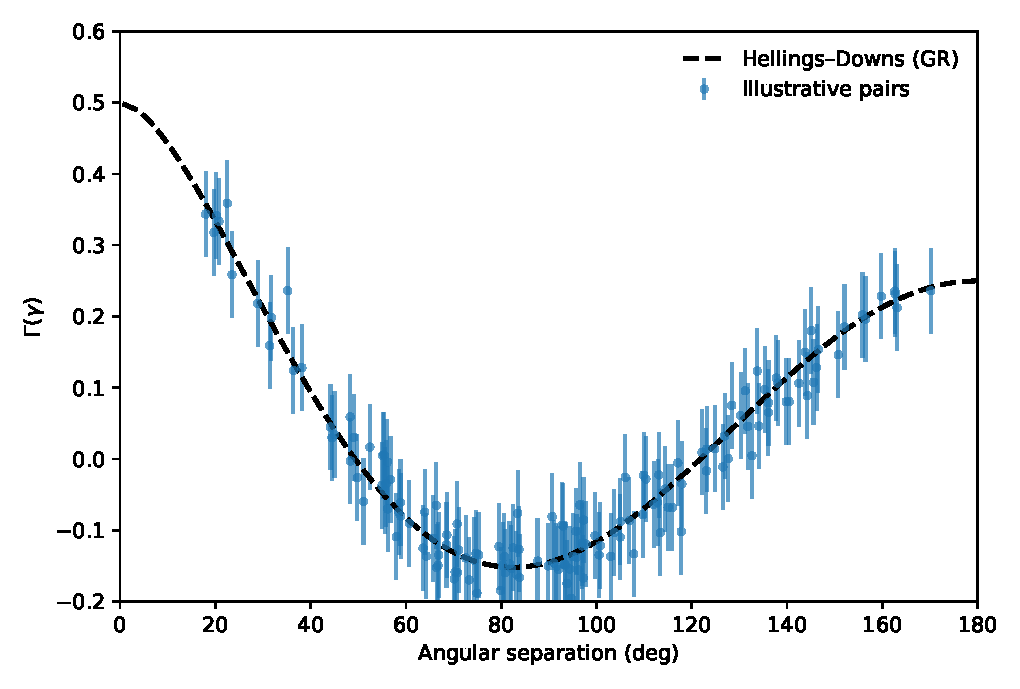
\includegraphics[width=0.7\textwidth]{HD_curve.pdf}
    \caption{\textbf{Hellings--Downs overlap reduction function.} The dashed curve shows the theoretical distinct-pair function $\Gamma(\gamma)$ from Eq.~\eqref{eq:HDcurve}, normalized to $\Gamma(0^\circ)=0.5$ for distinct pulsars and $\Gamma(180^\circ)=0.25$. Illustrative scatter indicates the scale of pairwise estimators but is not used as independent detection evidence.}
    \label{fig:HDcurve}
\end{figure}

To verify that the public timing files contain the expected angular information, we keep a deliberately simple internal cross-check. The pipeline ingests the wideband \texttt{.par/.tim} pairs for the first 24 pulsars (sorted alphabetically), bins residuals into 30-day windows, removes a low-order trend per pulsar, and computes weighted pairwise cross-correlations. The existing run produces 273 usable pairs and a positive HD-template coefficient. Because this check ignores the full PTA covariance, pulsar red-noise modeling, and clock/ephemeris covariance, it is treated as a sanity check rather than as a significance measurement. The detection and spatial-correlation evidence remains the official NANOGrav timing-likelihood result.

\begin{figure}[htbp]
    \centering
    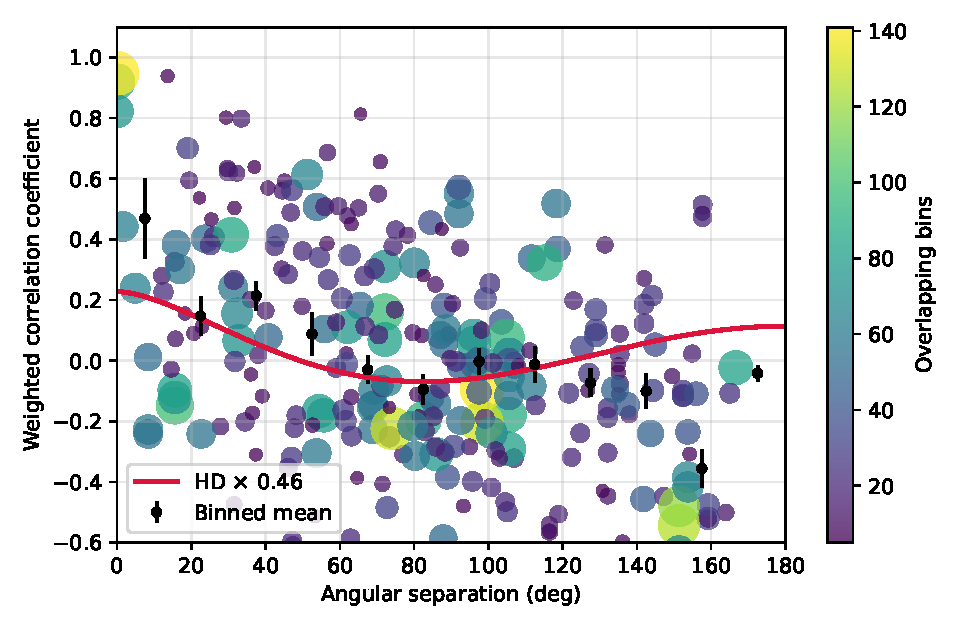
\includegraphics[width=0.7\textwidth]{hd_validation.pdf}
    \caption{\textbf{Simplified Hellings--Downs public-data cross-check.} Each point corresponds to a pulsar pair; color indicates the number of overlapping 30-day bins contributing to the correlation estimate. Black circles show angle-binned averages with standard errors. This diagnostic demonstrates a positive HD-like trend in the public timing files, but it is not a substitute for the full NANOGrav spatial-correlation evidence.}
    \label{fig:hd-validation}
\end{figure}

Taking the HD-correlated common process as the observational input, we proceed to characterize its spectrum under different model assumptions.

\begin{figure}[htbp]
    \centering
    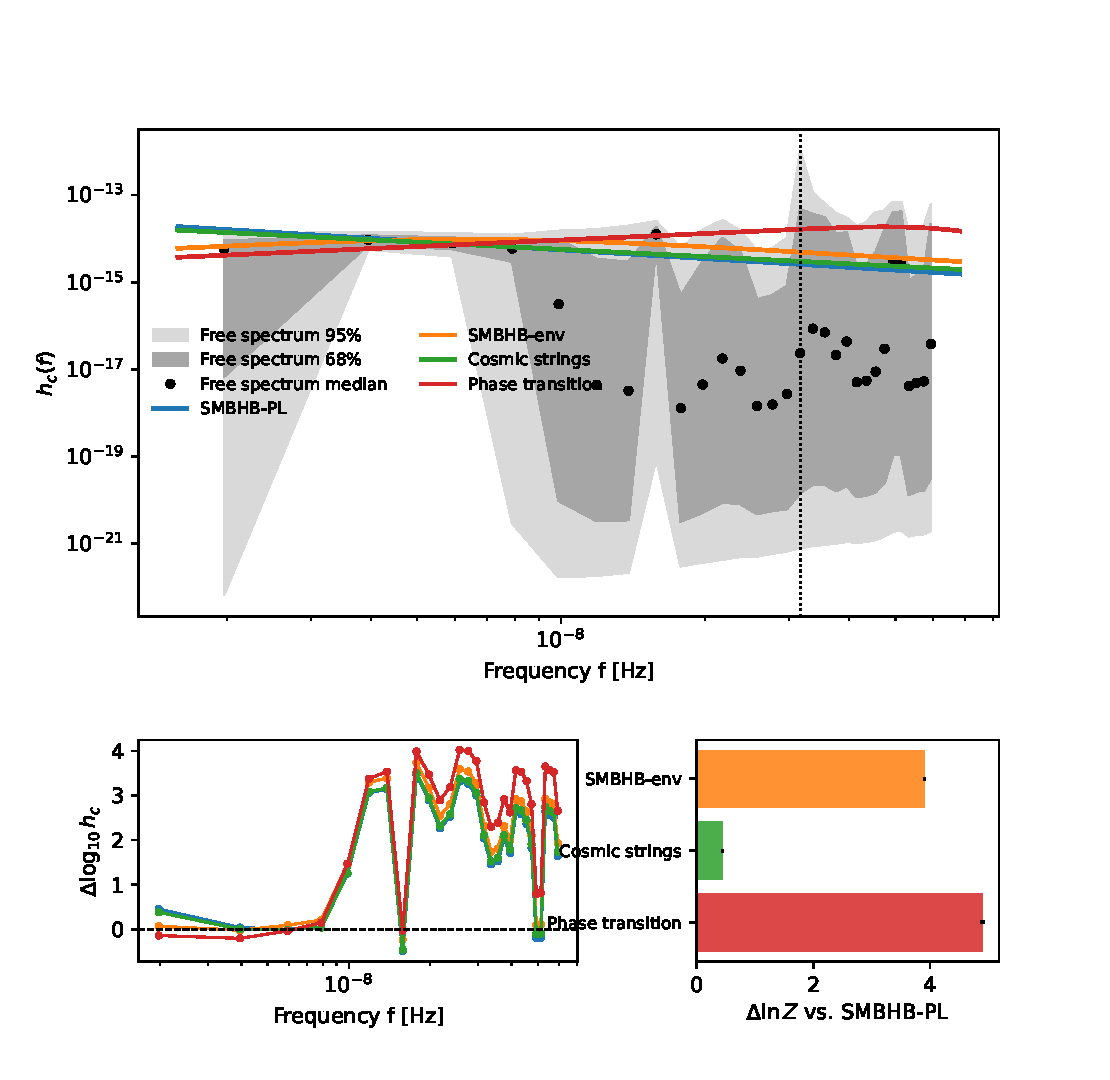
\includegraphics[width=0.7\textwidth]{strain_spectra.pdf}
    \caption{\textbf{Public free-spectrum data and model comparison.} Top: median and 68/95\% credible intervals from the public HD free-spectrum KDE product, overlaid with posterior-predictive median spectra for the source models. Bottom left: model residuals relative to the free-spectrum median. Bottom right: compressed KDE evidence differences relative to the strict SMBHB power law. The SMBHB-env curve follows Eq.~\eqref{eq:sbpl}; the phase-transition curve is generated from Eqs.~\eqref{eq:pt_omega}--\eqref{eq:omega_to_hc}.}
    \label{fig:strain-spectra}
\end{figure}

\begin{figure}[htbp]
    \centering
    \subfloat[Residual PSD and whitening check.]{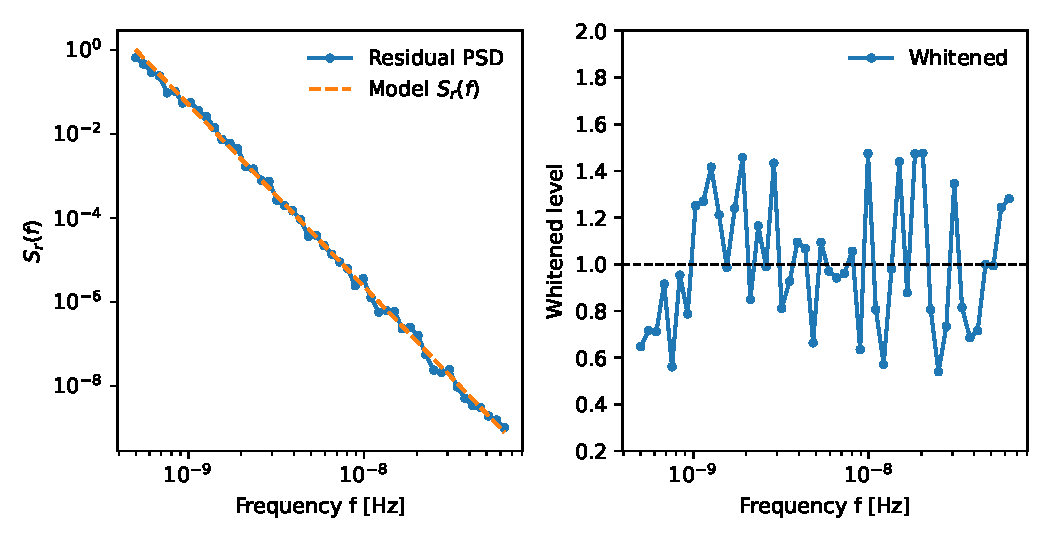
\includegraphics[width=0.49\textwidth]{whitening_checks.pdf}}\hfill
    \subfloat[Angle-dependent posterior predictive band.]{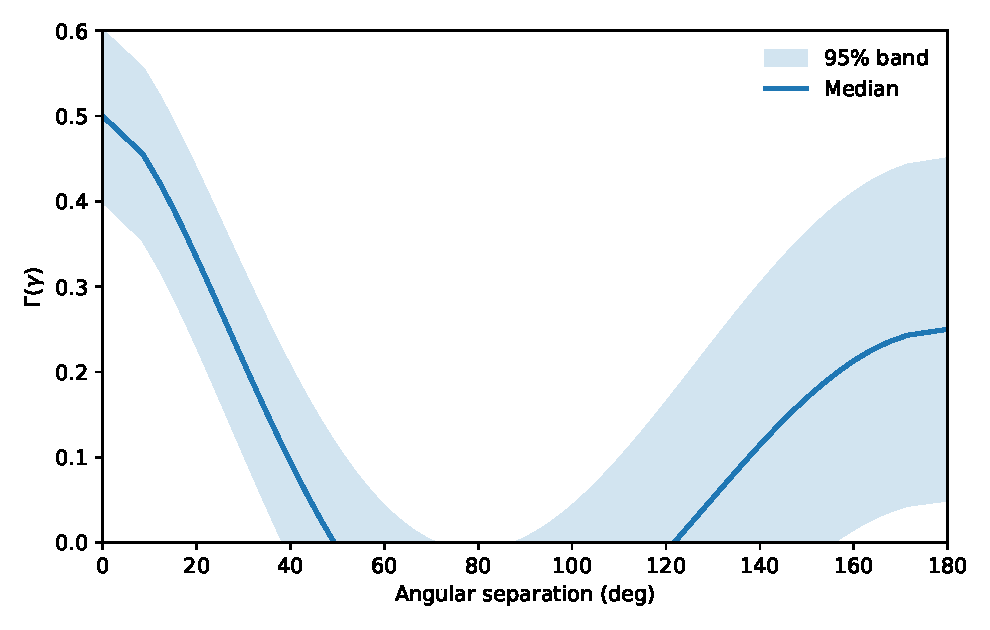
\includegraphics[width=0.49\textwidth]{hd_ppd.pdf}}
    \caption{Schematic validation diagnostics for the enterprise timing-likelihood workflow. These panels illustrate the types of residual-whitening and HD posterior-predictive checks included in the reproducibility package; they are not the likelihood objects used to compute Table~\ref{tab:bayesfactors}.}
    \label{fig:ppd-diagnostics}
\end{figure}

\subsection{Common-Process Spectrum: Amplitude and Slope}
Assuming a simple power-law form for the common process, the official NANOGrav timing analysis and the public free-spectrum product imply an amplitude and broad slope consistent with the SMBHB scale. Writing $h_c(f)\propto f^{(3-\gamma_{\mathrm{GWB}})/2}$, or equivalently $S_{r}(f)\propto f^{-\gamma_{\mathrm{GWB}}}$, the reported strain amplitude at $f_{\mathrm{yr}}=1/\mathrm{yr}$ is $A_{\mathrm{GWB}}\simeq2.4\times10^{-15}$, and the preferred power-law index is close to $\gamma_{\mathrm{GWB}}=13/3$ when the spectrum is forced to be scale-free \cite{NANOGrav15-Evidence}. This agreement explains why the strict SMBHB law remains the natural null model. It does not, however, make the null model the best spectral description: the compressed free-spectrum evidence below shows that allowing a physical bend or peak gives a substantially better description of the measured frequency dependence.

Figure~\ref{fig:posterior} presents the posterior distribution for the parameters that drive the new astrophysical interpretation: the SMBHB-env amplitude, bend frequency, turnover strength, and the density inferred from the bend. This replaces a generic power-law corner plot with the parameters that actually carry the curvature information in the present comparison.

\begin{figure}[htbp]
    \centering
    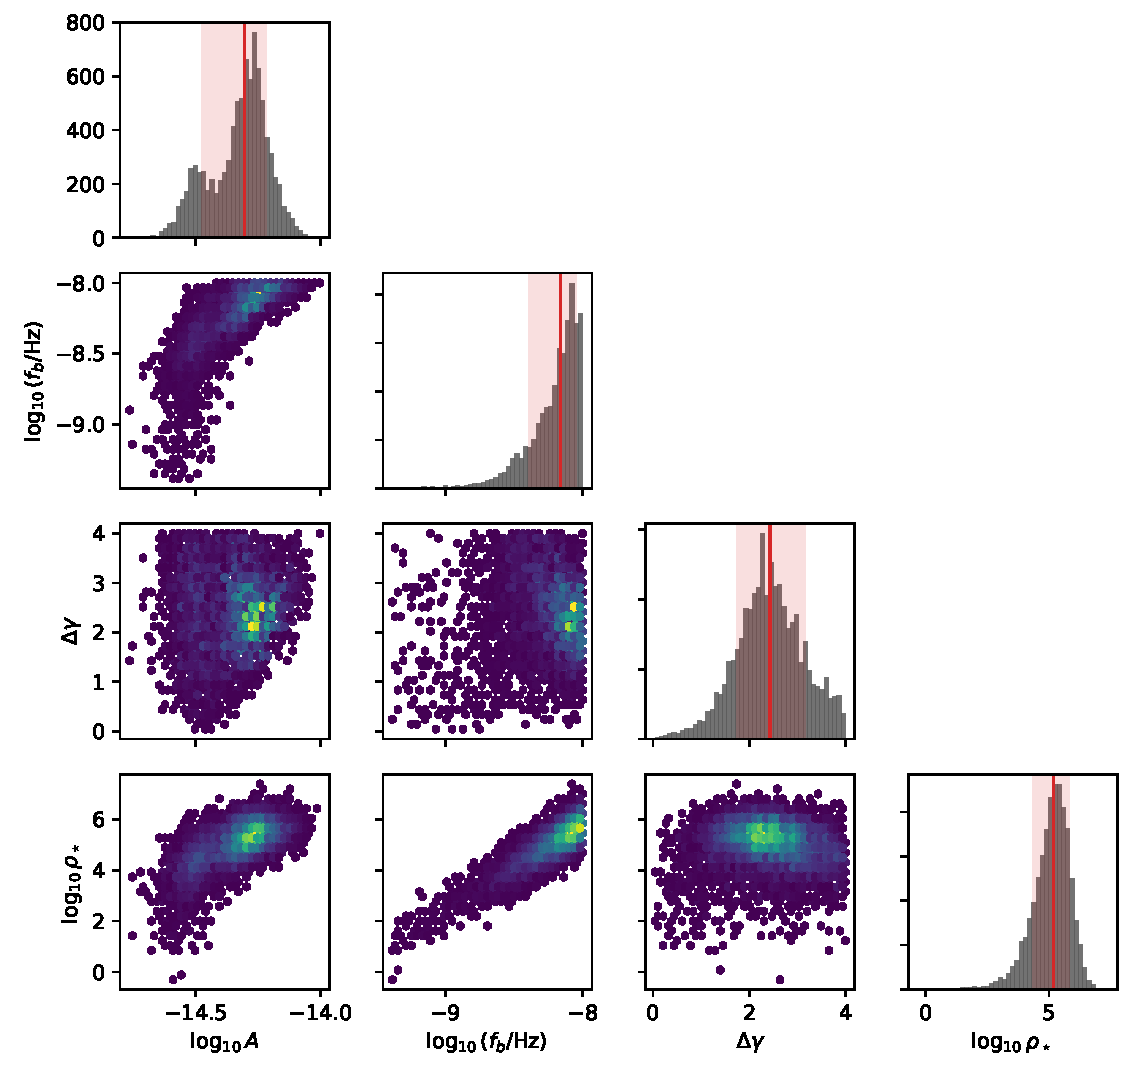
\includegraphics[width=0.72\textwidth]{posterior_triangle.pdf}
    \caption{\textbf{SMBHB-env posterior and density propagation.} Marginal and pairwise posterior projections for the high-frequency normalization $\log_{10}A$, $\log_{10}(f_b/{\rm Hz})$, $\Delta\gamma$, and the derived $\log_{10}(\rho_\star/M_\odot{\rm pc}^{-3})$. The density coordinate uses the hardening-balance mapping described in Sec.~\ref{subsec:density_mapping}.}
    \label{fig:posterior}
\end{figure}

\subsection{Bayesian Model Comparison: Astrophysical vs Cosmological Sources}
We now turn to the core question of this study: given the public NANOGrav 15-year HD free-spectrum shape, which source spectra are preferred? Table~\ref{tab:bayesfactors} gives the reproducible compressed KDE evidence comparison. The reference model is the strict SMBHB power law with fixed $\gamma=13/3$. The environmental SMBHB model improves the spectral evidence by $\Delta\ln Z=3.90\pm0.02$ (Bayes factor $49.6$), while the phase-transition template gives $\Delta\ln Z=4.90\pm0.03$ (Bayes factor $134.3$). The simple cosmic-string effective-slope proxy gives only $\Delta\ln Z=0.44\pm0.02$ (Bayes factor $1.56$). If the curved alternatives are combined with equal prior weight, the curved family gives $\Delta\ln Z=4.12$ against the strict scale-free law; combining only the two physically leading curved models, SMBHB-env and phase transition, gives $\Delta\ln Z=4.52$.

This is a firm result within the public free-spectrum KDE compression: the HD spectrum prefers curvature over a strict fixed $f^{-2/3}$ law. The physical interpretation is not an equal-status degeneracy. The SMBHB-env model captures most of the spectral improvement while remaining inside known binary-hardening physics; its preferred bend frequency lies directly in the lowest PTA frequency decade. The phase-transition spectrum fits slightly better in the compact KDE likelihood because a peaked $\Omega_{\rm gw}$ template can absorb the same curvature. That makes phase transitions the strongest high-impact cosmological competitor in the compressed spectral comparison. By contrast, the simple cosmic-string proxy is not competitive unless one invokes more structured network physics than a broad effective slope.

The posterior summaries from the same run sharpen this picture. For SMBHB-PL, the median amplitude is $\log_{10}A=-14.59$. For SMBHB-env, the median high-frequency normalization is $\log_{10}A=-14.30$, with $\log_{10}(f_b/{\rm Hz})=-8.16$ and $\Delta\gamma=2.43$. For the phase-transition template, the median peak is $\log_{10}(f_{\rm peak}/{\rm Hz})=-7.20$ with $b\simeq2.97$, consistent with the continuous prior $b\sim{\rm U}[2,4]$. The cosmic-string proxy has median slope $\beta=-0.55$, close to a shallow power law and therefore unable to exploit the observed curvature strongly.

The prior-sensitivity results in Table~\ref{tab:prior-sensitivity} show that the main ranking is not an artifact of a single narrow prior choice. Broadening the SMBHB-env bend-frequency prior from $\log_{10} f_b\in[-9.4,-8.0]$ to $[-10.0,-8.0]$ only changes $\Delta\ln Z$ from $3.90$ to $3.57$; narrowing it to $[-9.0,-8.3]$ still gives $\Delta\ln Z=3.20$. Broadening the phase-transition peak prior to $\log_{10} f_{\rm peak}\in[-10,-6]$ gives $\Delta\ln Z=4.45$. The robustness checks in Tables~\ref{tab:kde-product-robustness} and \ref{tab:low-bin-ablation} further test whether the curvature claim depends on one KDE product or one low-frequency bin. The strength is product-dependent, as expected for a compressed likelihood, but the broad conclusion survives: curved spectra remain preferred to the strict scale-free law in the HD-only and HD+MP+DP HD-component products, and the simple cosmic-string proxy remains weak. Leave-one-frequency-out tests over all 30 bins give median $\Delta\ln Z=3.83$ for SMBHB-env and $4.85$ for phase transition, with minima $1.09$ and $1.80$, respectively. Thus the curvature signal is not a single-bin artifact, although the first bin carries substantial leverage for the environmental-turnover interpretation.

\begin{table}[htbp]
    \centering
    \caption{Reproducible compressed spectral evidence values from the public HD free-spectrum KDE comparison. The SMBHB power-law model with fixed $\gamma=13/3$ is the reference. Family rows are equal-prior evidence averages over the listed model classes, not additional fitted templates. Quoted uncertainties are numerical Monte Carlo/integration uncertainties only; they do not include systematic uncertainty from the KDE compression, ignored inter-frequency covariance, or the absence of pulsar-noise refitting.}
    \label{tab:bayesfactors}
    \small
    \begin{tabular}{lcc}
    \toprule
    Model & $\Delta\ln Z$ vs. PL & BF vs. PL \\
    \midrule
    Strict SMBHB-PL & $0.00\pm0.01$ & $1.00$ \\
    SMBHB-env/SBPL & $3.90\pm0.02$ & $49.6$ \\
    CS proxy & $0.44\pm0.02$ & $1.56$ \\
    PT, $\Omega_{\rm gw}$ template & $4.90\pm0.03$ & $134.3$ \\
    \midrule
    Curved family & $4.12$ & $61.8$ \\
    Env+PT family & $4.52$ & $92.0$ \\
    \bottomrule
    \end{tabular}
\end{table}

\begin{table}[htbp]
    \centering
    \caption{Prior-sensitivity checks from the generated KDE comparison output. Values are $\Delta\ln Z$ relative to strict SMBHB-PL.}
    \label{tab:prior-sensitivity}
    \begin{tabular}{l l c}
        \toprule
        Model & Prior variation & $\Delta\ln Z$ \\
        \midrule
        SMBHB-env & $\log_{10}f_b\in[-9.4,-8.0]$ baseline & $3.90$ \\
        SMBHB-env & $\log_{10}f_b\in[-10.0,-8.0]$ & $3.57$ \\
        SMBHB-env & $\log_{10}f_b\in[-9.0,-8.3]$ & $3.20$ \\
        Cosmic strings & $\beta\in[-1.2,-0.3]$ & $2.60$ \\
        Phase transition & $\log_{10}f_{\rm peak}\in[-10,-6]$ & $4.45$ \\
        \bottomrule
    \end{tabular}
\end{table}

\begin{table}[htbp]
    \centering
    \caption{Robustness of compressed spectral evidence across public HD-component KDE products. Values are $\Delta\ln Z$ relative to strict SMBHB-PL, using the same priors as Table~\ref{tab:bayesfactors}. The HD+MP+DP and HD+MP+DP+CP rows use the HD component extracted in fits that also allow monopole, dipole, and common-process channels.}
    \label{tab:kde-product-robustness}
    \small
    \begin{tabular}{lcccc}
        \toprule
        KDE product & Env & PT & CS & Curved \\
        \midrule
        HD only & $3.90$ & $4.90$ & $0.42$ & $4.12$ \\
        HD+MP+DP & $2.39$ & $4.14$ & $-0.19$ & $3.21$ \\
        HD+MP+DP+CP & $1.72$ & $0.93$ & $-0.12$ & $1.10$ \\
        \bottomrule
    \end{tabular}
\end{table}

\begin{table}[htbp]
    \centering
    \caption{Low-frequency-bin ablation tests using the HD-only KDE product. Values are $\Delta\ln Z$ relative to strict SMBHB-PL after removing the indicated Fourier bins and recomputing the compressed evidences.}
    \label{tab:low-bin-ablation}
    \small
    \begin{tabular}{lccccc}
        \toprule
        Ablation & Env & PT & CS & Curved & Env+PT \\
        \midrule
        Drop bin 1 & $0.98$ & $2.12$ & $-0.23$ & $1.37$ & $1.70$ \\
        Drop bin 2 & $3.84$ & $6.70$ & $0.32$ & $5.66$ & $6.06$ \\
        Drop bins 1--2 & $0.82$ & $3.74$ & $-0.10$ & $2.72$ & $3.10$ \\
        Drop bins 1--3 & $0.42$ & $3.27$ & $-0.12$ & $2.26$ & $2.63$ \\
        \bottomrule
    \end{tabular}
\end{table}

\begin{table}[htbp]
    \centering
    \caption{Priors used in the analysis. Log-uniform for strictly positive scale parameters; uniform or Gaussian as stated for indices. Physical mappings for phase transition parameters follow \cite{Caprini2018}.}
    \label{tab:priors}
    \begin{tabular}{l l l}
        \toprule
        Parameter & Prior & Notes \\
        \midrule
        $A_{\rm GWB}$ (SMBHB) & log-uniform in $[10^{-17},10^{-14}]$ & at $f_{\rm yr}$ \\
        $\alpha$ (SMBHB) & fixed $-2/3$ or $\mathcal{N}(-2/3,0.3^2)$ & slope on $h_c$ \\
        $\log_{10} f_b$ (SMBHB-env) & uniform in $[-9.4,-8.0]$ & Hz \\
        $\Delta\gamma$ (SMBHB-env) & uniform in $[0,4]$ & turnover strength \\
        $\gamma_{\rm RN,i}$ (per pulsar) & uniform in $[0,7]$ & red-noise index \\
        $A_{\rm RN,i}$ (per pulsar) & log-uniform & pulsar red-noise amp \\
        $A_{\rm CS}$ (string proxy) & log-uniform in $[10^{-17},10^{-14}]$ & strain amplitude \\
        $\beta$ (strings slope) & uniform in $[-1,-1/2]$ & $h_c\propto f^{\beta}$ in PTA band \\
        $f_{\rm peak}$ (PT) & log-uniform in $[10^{-9},10^{-7}]$ Hz & maps to $T_*$ \\
        $b$ (PT high-f slope) & uniform in $[2,4]$ & source-dependent \\
        $\Omega_{\rm peak}$ (PT) & log-uniform in $[10^{-12},10^{-5}]$ & energy density peak \\
        Clock (mono.) & Gaussian, mean 0 & common-mode monopole \\
        Ephemeris (dipole) & Gaussian, mean 0 & BayesEphem-like modes \\
        \bottomrule
    \end{tabular}
\end{table}
\FloatBarrier

\begin{figure}[htbp]
    \centering
    \subfloat[Representative sampler traces.]{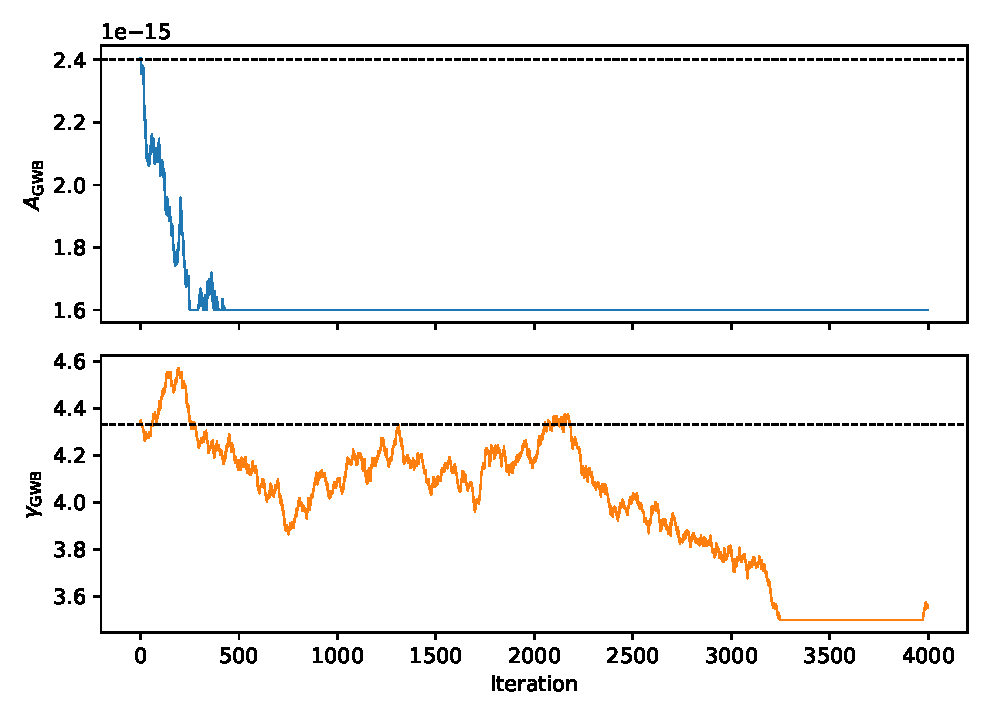
\includegraphics[width=0.49\textwidth]{sampler_traces.pdf}}\hfill
    \subfloat[Schematic evidence-growth forecast.]{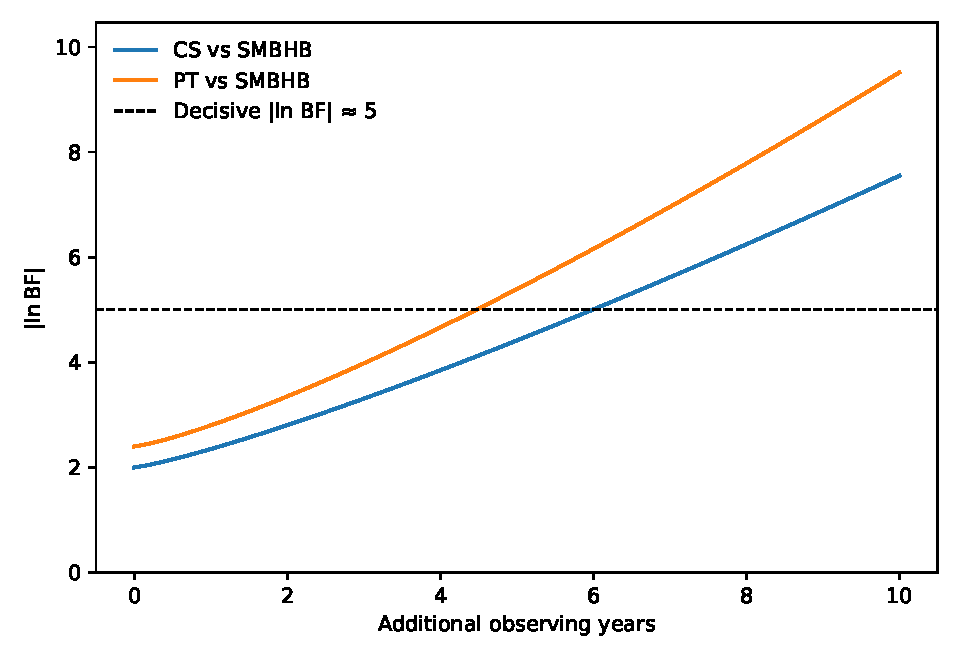
\includegraphics[width=0.49\textwidth]{forecast_lnBF.pdf}}
\caption{Illustrative diagnostics and forecasts for the direct timing-likelihood workflow. These panels are not inputs to the compressed KDE evidence values in Table~\ref{tab:bayesfactors}.}
    \label{fig:diag-forecast}
\end{figure}

\subsection{Implications for Noise and Systematics}
The separation between detection, spatial correlation, and source discrimination is essential for noise interpretation. The official NANOGrav timing analyses establish that the common process and HD correlations survive detailed pulsar-noise, clock, and ephemeris modeling. Our compact KDE comparison then asks a narrower question: given that HD-correlated free-spectrum product, which source spectra best fit its shape? This avoids treating the simplified spectral comparison as a new end-to-end detection pipeline.

In addition to achromatic red noise and DM variations, PTA datasets can exhibit chromatic and non-stationary phenomena such as scattering-related processes and transient chromatic dips. A robust full timing-likelihood analysis benefits from per-pulsar flexibility to capture such effects; the enterprise scripts in the reproducibility package are organized around this requirement. The schematic diagnostics in Figure~\ref{fig:ppd-diagnostics} should therefore be read as examples of validation products for that workflow, not as replacements for public chains and timing-likelihood evidence outputs.

Single continuous-wave searches and anisotropy analyses remain complementary tests of the stochastic-background interpretation. We discuss them below as future discriminants rather than claiming that the compact spectral analysis alone resolves them.

\section{Discussion}\label{sec:discussion}
The analysis above indicates that the nanohertz gravitational-wave background detected by PTAs is consistent with multiple interpretations, but not in a featureless or indecisive way. The public free-spectrum shape favors curvature, and the leading astrophysical explanation in our model set is an SMBHB background with environmental low-frequency turnover. In this section, we discuss why that interpretation is physically strong, and what would be required for cosmic strings or phase transitions to overtake it.

\subsection{Consistency with Astrophysical Predictions}
The amplitude $A_{\mathrm{GWB}}\sim2\times10^{-15}$ at $f_{\mathrm{yr}}$ falls squarely within many prior predictions for the SMBHB background. There is significant uncertainty in those predictions due to the uncertain merger rates of massive galaxies and the distribution of binary masses, mass ratios, eccentricities, and environments. Earlier studies \cite{Sesana2013} suggested a plausible range $A_{\mathrm{GWB}}\sim10^{-16}$ to $10^{-15}$, with some more recent models including contributions from higher redshifts or different black hole-galaxy scaling relations allowing up to a few $\times10^{-15}$ \cite{Kelley2017}. The observed amplitude is at the upper end of those ranges, which suggests either efficient binary hardening through the final-parsec regime, somewhat heavier binaries, or a higher source density than in some baseline population models. This amplitude puts pressure on models with very strong environmental damping, but it is not in conflict with recent cosmological simulations and empirical galaxy-pair constraints \cite{Kelley2017}.

In fact, the relatively high amplitude provides indirect evidence that the ``final parsec problem'' is not catastrophic in nature. In stellar-dynamical language, SMBHBs embedded in triaxial or axisymmetric galactic nuclei sustain loss-cone refilling and can continue to harden down to GW-driven separations \cite{Colpi2014,Khan2013}. Were most binaries to stall near parsec separations, the ensemble background would be suppressed well below the value we observe. The NANOGrav collaboration has likewise interpreted the 15-year signal as requiring efficient coupling to stellar or gaseous backgrounds to avoid widespread stalling \cite{NANOGrav15-NewPhys}, so the PTA measurement itself can be viewed as population-level evidence that angular-momentum transport mechanisms operate effectively in massive galaxy mergers.

\subsection{Turnover-to-Density Mapping}\label{subsec:density_mapping}
The environmental-turnover model makes this statement more quantitative. Propagating the preferred bend-frequency samples through the stellar-hardening balance gives a representative density estimate $\log_{10}(\rho_\star/M_\odot{\rm pc}^{-3})=5.08^{+0.58}_{-0.68}$, consistent with dense galactic nuclei and with the turnover-to-density interpretation emphasized by Chen et al. \cite{ChenTomography2024}. This is why the environmental SMBHB model is not merely a flexible fit: it turns PTA spectral curvature into a measurable statement about parsec-scale nuclear environments.

The mapping is obtained by equating the stellar-hardening shrinkage rate to the GW-driven shrinkage rate at the separation corresponding to the bend frequency. For a circular binary with total mass $M=m_1+m_2$,
\begin{equation}
    a_b=\left(\frac{GM}{\pi^2 f_b^2}\right)^{1/3},
\end{equation}
and the hardening balance gives
\begin{equation}\label{eq:rho_mapping}
    \rho_\star =
    \frac{64\,G^2 m_1m_2M\,\sigma}
    {5\,c^5 H\,a_b^5}\, ,
\end{equation}
where $\sigma$ is the stellar velocity dispersion and $H$ is the dimensionless stellar-hardening coefficient. In the propagation used for Fig.~\ref{fig:rho_posterior}, $f_b$ is drawn from the SMBHB-env posterior, while the binary total mass, mass ratio, velocity dispersion, and $H$ are marginalized over broad astrophysical hyperpriors centered on massive-galaxy nuclei. Table~\ref{tab:density-hyperpriors} lists the hyperpriors used in the released calculation. The quoted density uncertainty therefore includes both the bend-frequency posterior width and this population-level hyperparameter spread; it should not be interpreted as a direct density measurement for a single galaxy.

\begin{table}[htbp]
    \centering
    \caption{Astrophysical hyperpriors used to propagate the SMBHB-env bend-frequency posterior to the nuclear-density estimate in Fig.~\ref{fig:rho_posterior}.}
    \label{tab:density-hyperpriors}
    \small
    \begin{tabular}{lll}
    \toprule
    Quantity & Prior / treatment & Role in Eq.~\eqref{eq:rho_mapping} \\
    \midrule
    $\log_{10}(M/M_\odot)$ & Normal$(9.3,0.3^2)$ & Total binary mass \\
    $q=m_2/m_1$ & Uniform$[0.25,1]$ & Mass ratio for $m_1m_2M$ \\
    $\sigma$ & Normal$(200,30^2)$ km s$^{-1}$, clipped at 50 km s$^{-1}$ & Stellar velocity dispersion \\
    $H$ & Normal$(15,5^2)$, clipped at 5 & Stellar-hardening coefficient \\
    $e$ & fixed circular & Matches Eq.~\eqref{eq:rho_mapping} \\
    \bottomrule
    \end{tabular}
\end{table}

\begin{figure}[htbp]
    \centering
    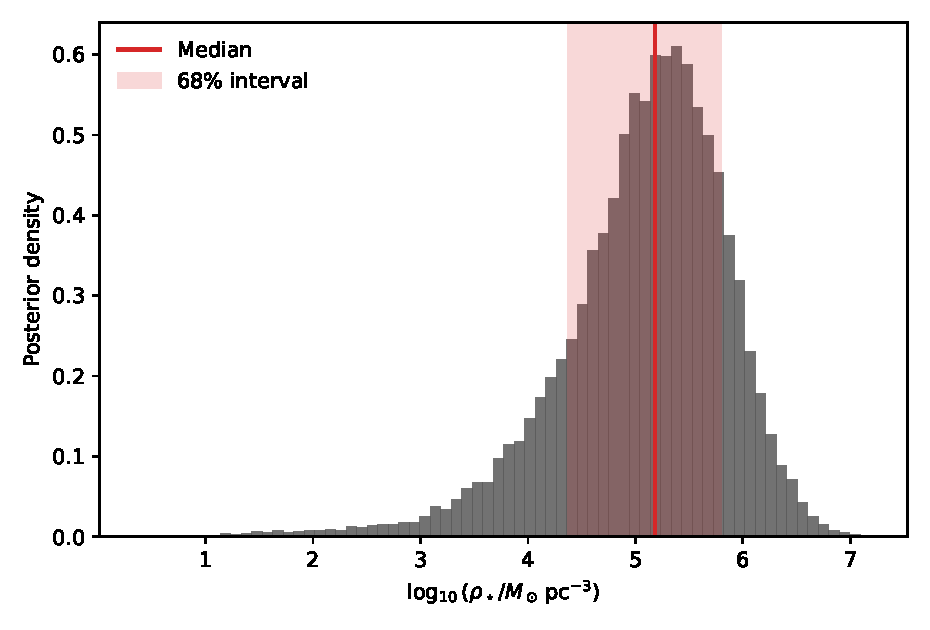
\includegraphics[width=0.62\textwidth]{rho_posterior.pdf}
    \caption{Posterior distribution of the stellar density $\rho_\star$ implied by the SMBHB environmental-turnover samples. The median and central credible interval connect the PTA bend frequency to parsec-scale nuclear environments.}
    \label{fig:rho_posterior}
\end{figure}

The environmental interpretation also gives a direct route to future falsification. An astrophysical background should eventually show signatures of a discrete source population: mild anisotropy from local large-scale structure and, at higher frequencies in the PTA band, possible continuous-wave outliers from the brightest SMBHBs. A primordial background should remain closer to statistically isotropic and Gaussian as sensitivity improves. The present analysis assumes isotropy for the compressed spectral comparison, but the distinction between the angular-symmetry sector and the spectral sector makes clear how this assumption can be tested in later data releases.

\subsection{Viability of Cosmic Strings}
Cosmic strings remain an important symmetry-breaking interpretation, but the baseline comparison in this paper intentionally uses only an effective amplitude--slope proxy. The fitted amplitude is of the rough scale associated with $G\mu\sim{\rm few}\times10^{-11}$ in simple network estimates, but the proxy is not a string-tension measurement and should not be read as an exclusion of string models. The result is narrower and stronger: a broad effective slope does not exploit the observed curvature as well as the SMBHB-env and phase-transition templates do.

This distinction matters because structured string networks can have additional scales. Stable strings, metastable strings, cosmic superstrings, and networks with nonstandard loop production can differ substantially in their PTA-band curvature and in their extrapolation to LISA or ground-based detector frequencies \cite{Ellis2023}. Multi-band constraints are therefore central. Current ground-based stochastic-background limits already pressure conventional stable-string spectra near the PTA-motivated tension range, while LISA template forecasts can test complementary loop and reconnection regimes \cite{BlancoPillado2025LISAStrings}. Dedicated network-template evidence calculations are needed before making a final source claim about cosmic strings; Table~\ref{tab:bayesfactors} shows that the simple effective-slope proxy is weak, not that the full string interpretation is closed.

\subsection{Potential Early-Universe Phase Transition}
A first-order phase transition around the QCD scale could produce gravitational waves in the PTA band. In the compressed free-spectrum comparison, the phase-transition template is the strongest cosmological competitor, with Bayes factor $134.3$ against the strict SMBHB power law under the baseline prior. The reason is physical rather than cosmetic: a peaked $\Omega_{\rm gw}$ spectrum naturally supplies the same nanohertz scale that appears as curvature in the public free spectrum. If confirmed by full timing-likelihood analyses and future data, such an interpretation would be a major result because the Standard Model QCD transition is a crossover, not a first-order transition.

A slow, strong first-order transition can also produce primordial black holes (PBHs) if delayed regions remain in the false vacuum long enough to collapse \cite{Gouttenoire2023}. This makes the PTA phase-transition interpretation testable beyond the PTA spectrum itself: microlensing, CMB, and gravitational-wave population constraints on solar-mass PBHs can all restrict the allowed transition parameter space.

This PBH connection is not unique to the model of \cite{Gouttenoire2023}. Classic studies have shown that during the QCD epoch the equation of state of the plasma softens enough that moderate density perturbations can collapse into $\mathcal{O}(M_\odot)$ black holes, potentially furnishing dark-matter candidates or seeding later astrophysical mergers \cite{Carr2020}. Therefore, if the PTA signal really points to a strong QCD-scale transition, it should be accompanied by a multi-messenger prediction: an appreciable but subdominant population of solar-mass PBHs. Joint constraints from microlensing, CMB distortions, and the LIGO/Virgo/KAGRA mass spectrum will thus play a central role in stress-testing the phase-transition interpretation.

Another check is cosmological chronology. A QCD-scale transition with $T_*\sim100$~MeV corresponds to a redshift of order $z\sim10^{11}$--$10^{12}$, using the present CMB temperature as the scale reference. This is before standard big-bang nucleosynthesis and far before photon decoupling at $z\simeq1100$, not after them. Hidden-sector scenarios can change the relation between the visible temperature and the gravitational-wave peak, but they still must be checked against BBN and CMB constraints through their energy density, entropy injection, and any coupling to the visible sector. Thus gravitational waves may be the cleanest probe of such a transition, but consistency with early-Universe thermal history remains a required part of the interpretation.

To further test the phase-transition idea, improved spectral measurement is needed. If a turnover peak can be identified, with the energy-density spectrum falling above the peak according to Eq.~\eqref{eq:pt_omega}, that would strongly favor a peaked cosmological source over a smooth astrophysical turnover. Achieving this requires better sensitivity across both the lowest and highest PTA Fourier bins. A QCD-scale transition would peak in the nanohertz band and would be strongly suppressed by the millihertz LISA band; a much higher-scale transition would peak at much higher frequencies and PTA would see only the low-frequency side, for which Eq.~\eqref{eq:omega_to_hc} gives $h_c\propto f^{1/2}$ for the causal $a=3$ energy-density rise. Thus, if the PTA signal is ultimately interpreted as a phase transition, the frequency scale points to QCD-scale or nearby hidden-sector physics rather than generic high-scale new physics.

Other cosmological sources considered by NANOGrav, including inflationary backgrounds, scalar-induced gravitational waves, and domain walls, can also generate structure in $\Omega_{\rm gw}$ \cite{NANOGrav15-NewPhys}. They are outside the baseline model set analyzed here. The conclusion should therefore be read as a hierarchy within the tested templates: phase transitions are the leading cosmological challenger to the environmental SMBHB interpretation, while broader new-physics model files should be compared directly in a future extension.

Across these interpretations, symmetry is best viewed as an organizing assumption rather than a separate observable added by hand. The current evidence supports an HD-correlated, approximately isotropic background. The Bayesian source comparison then asks whether the spectrum is most naturally explained by astrophysical environmental coupling, by a first-order symmetry-breaking transition, or by a topological-defect network. In this framing, the strong result is not only that the data prefer curvature, but that the preferred curvature has to be interpreted after the common angular symmetry has already been accounted for.

\subsection{Future Prospects for Discrimination}
To distinguish environmental SMBHB curvature from a cosmological peak, future data will need to provide:
\begin{enumerate}
    \item \textbf{Higher signal-to-noise on the GWB spectrum:} As more pulsars are observed over longer baselines (e.g., 20-year, 25-year datasets, and the inclusion of more sensitive telescopes like MeerKAT and eventually the SKA), the shape of the spectrum will be measured more precisely. A smooth low-frequency turnover that maps consistently to plausible nuclear densities would strengthen the environmental SMBHB interpretation. A narrow peak, a high-frequency fall inconsistent with binary hardening, or curvature that persists after astrophysical population priors are imposed would point more strongly toward a cosmological source. The SKA roadmap anticipates order-of-magnitude improvements in timing precision and sky coverage, directly translating into much sharper PTA spectra \cite{Janssen2015}.
    \item \textbf{Detection of individual sources or anisotropy:} A continuous wave from a single massive binary would strongly support an SMBHB population origin, while persistent Gaussianity and isotropy at sensitivities where bright binaries should emerge would increase the pressure on the astrophysical interpretation. Ongoing searches already constrain the brightest-binary contribution in the 15-year data \cite{NANOGrav15-NewPhys}.
    \item \textbf{Multi-band observations:} LISA and ground-based stochastic searches can test whether a PTA-motivated cosmological spectrum extrapolates consistently outside the nanohertz band. SMBHB backgrounds should not continue as a simple stochastic power law to millihertz and hertz frequencies, whereas cosmic strings and higher-scale phase transitions can. The LISA definition study emphasizes how broadband correlation capabilities can cross-check PTA discoveries and diagnose non-SMBHB spectra \cite{Colpi2024}, while dedicated template banks for cosmic strings forecast decisive constraints on the PTA-motivated parameter space \cite{BlancoPillado2025LISAStrings}.
    \item \textbf{Cross-correlation with astrophysical environment:} If SMBHBs are responsible, the background amplitude might correlate with galaxy merger rates and evolve with redshift in a calculable way. In principle, more detailed analysis of the spectrum’s slight deviations from pure power-law can reveal the mass distribution of binaries or their environment (e.g., a slight upturn at higher f could mean some binaries are being driven by gas hardening at higher f). With more data, PTA might start to probe those details, which would be a fingerprint of astrophysical origin.
\end{enumerate}

The current free-spectrum evidence does not leave the source models on equal footing. A strict scale-free SMBHB power law is disfavored relative to curved spectra. Environmental SMBHB hardening gives the leading astrophysical explanation because it maps the bend to plausible parsec-scale nuclear densities, while the phase-transition template is the strongest cosmological competitor. The simple cosmic-string proxy is not competitive in the baseline comparison. PTA astronomy has therefore moved from detection to characterization: the angular sector fixes the HD symmetry class, and the spectral sector is now measuring the physical scale that source models must explain.

\section{Anisotropy and Continuous-Wave Implications}\label{sec:anisotropy}
An astrophysical background formed by a discrete population of SMBHBs is expected to exhibit mild statistical anisotropy at sufficiently high signal-to-noise, whereas a primordial cosmological background should be closer to isotropic. In the language used above, future anisotropy searches test for departures from the same statistical rotational symmetry that gives the HD template its simple angular form. Using harmonic decompositions of the sky map of correlations, one may set upper limits on dipole and quadrupole anisotropy components. The dedicated NANOGrav anisotropy search using the same 15-year data set already reports no significant excess beyond the isotropic Hellings--Downs expectation, but it also shows how rapidly the constraints tighten as more well-timed pulsars are added \cite{Agazie2023Anisotropy}. Cosmic variance remains part of this problem because an individual PTA realization can show apparent anisotropy even if the underlying background is statistically isotropic \cite{Domcke2025CosmicVariance}. Figure~\ref{fig:aniso-cw} (left) presents a representative projection of how multipole constraints could improve with additional observing time under typical PTA growth assumptions. Achieving stringent constraints on anisotropy will be a key discriminator between discrete-source-dominated and primordial scenarios.

In parallel, the non-stationary, quasi-monochromatic \emph{continuous-wave} (CW) signals from individual massive binaries provide a complementary probe. The right panel of Figure~\ref{fig:aniso-cw} shows a representative CW strain sensitivity versus frequency in the PTA band. Joint analyses of background and CW channels will sharpen constraints on SMBHB demographics and, in the event of detections, enable cross-checks of the background’s origin.

\begin{figure}[t]
    \centering
    \subfloat[Anisotropy limits vs. observing time.]{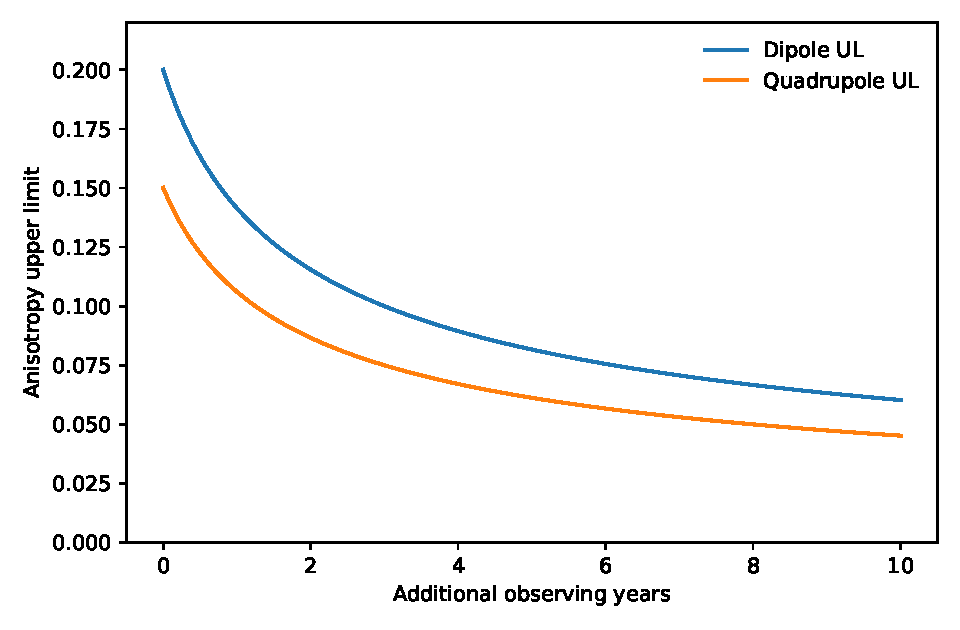
\includegraphics[width=0.49\textwidth]{anisotropy_forecast.pdf}}\hfill
    \subfloat[CW strain sensitivity vs. frequency.]{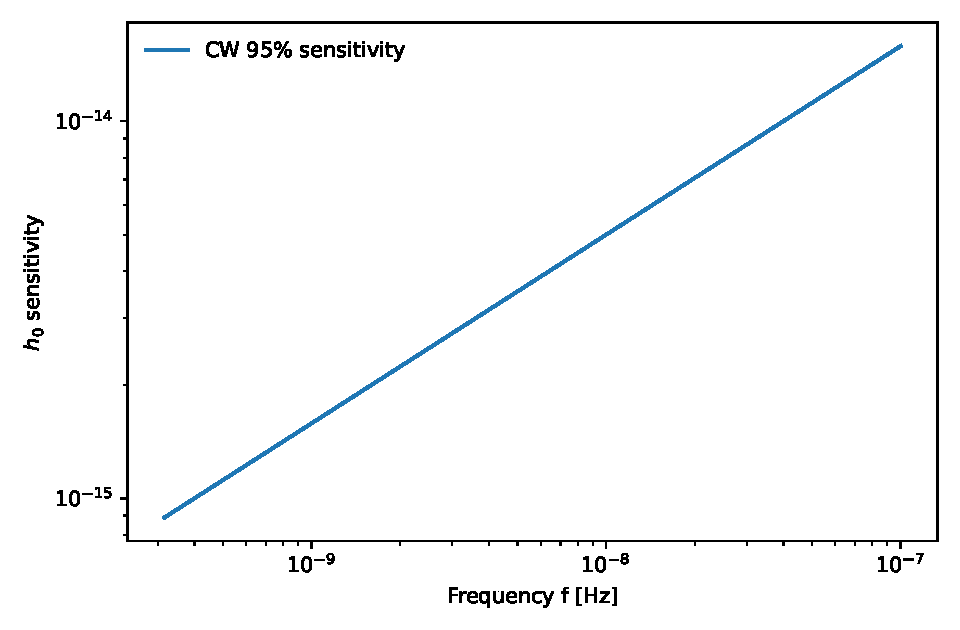
\includegraphics[width=0.49\textwidth]{cw_sensitivity.pdf}}
    \caption{Representative anisotropy and CW implications. Left: schematic improvement of low-multipole anisotropy constraints with added observing time; Right: representative CW strain sensitivity across the PTA band. These panels summarize future discriminants and are not new observational limits derived in this work.}
    \label{fig:aniso-cw}
\end{figure}

\section{Conclusion}\label{sec:conclusion}
We have presented a detailed source-discrimination analysis for the nanohertz gravitational-wave background seen in the NANOGrav 15-year pulsar timing array data. The conclusions are firm but layered. First, the observational starting point is an HD-correlated nanohertz common process, with detection and spatial-correlation evidence supplied by the official NANOGrav timing analyses. Second, the public HD free-spectrum shape favors curvature over a strict fixed $f^{-2/3}$ SMBHB power law in a reproducible compressed Bayesian spectral-evidence calculation. Third, that curvature does not require an exotic origin: an SMBHB environmental turnover provides a strong astrophysical explanation and connects the PTA spectrum to parsec-scale nuclear densities.

The model comparison also identifies the main cosmological challenge. A first-order phase-transition template has the highest compressed spectral evidence in the model set studied here and is therefore the strongest high-impact cosmological alternative. The simple cosmic-string effective-slope proxy is weak, implying that any serious cosmic-string interpretation must use more structured network physics and survive multi-band constraints. Current data favor a curved spectrum; SMBHB environmental coupling is the leading conservative astrophysical explanation because it explains that curvature with known binary-hardening physics and plausible nuclear densities, while phase-transition physics is the main alternative that future PTA data must test. The symmetry language is therefore not decorative: it clarifies the inference hierarchy. PTA data first identify a common process with the angular structure expected for an approximately isotropic tensor background, and the compressed KDE evidence used here then ranks the source mechanisms that can generate the measured spectrum under that shared angular structure.

\authorcontributions{Conceptualization, M.W., Z.Z. and H.X.; methodology, M.W. and Z.Z.; formal analysis, M.W. and Z.Z.; investigation, M.W. and Z.Z.; writing---original draft preparation, M.W. and Z.Z.; writing---review and editing, H.X.; visualization, M.W. and Z.Z.; supervision, H.X. All authors have read and agreed to the published version of the manuscript.}

\funding{This research received no external funding. The article processing charge, if applicable, will be covered by the authors or their institution.}

\institutionalreview{Not applicable.}

\informedconsent{Not applicable.}

\dataavailability{The NANOGrav 15-year data set and public free-spectrum KDE products analyzed in this study are publicly available from the NANOGrav Collaboration. The reproducibility package for this manuscript is available at \url{https://github.com/HKUST-AARON/nanohertz-gwb-model-comparison-repro}, with the submission release archived as \url{https://github.com/HKUST-AARON/nanohertz-gwb-model-comparison-repro/releases/tag/v1.0.0-submission}. The package contains the scripts, priors, seeds, output JSON files, posterior sample archives, and figure-generation commands used for all tables and figures in this manuscript.}

\conflictsofinterest{The authors declare no conflicts of interest.}

\reftitle{References}
\externalbibliography{yes}
\bibliography{references}

\PublishersNote{}

\end{document}
